%% LyX 2.4.3 created this file.  For more info, see https://www.lyx.org/.
%% Do not edit unless you really know what you are doing.
\documentclass[journal,article,submit,pdftex,moreauthors]{Definitions/mdpi}
\usepackage[utf8]{inputenc}
\usepackage{float}
\usepackage{url}
\usepackage{amsmath}
\usepackage{graphicx}

\makeatletter

%%%%%%%%%%%%%%%%%%%%%%%%%%%%%% LyX specific LaTeX commands.

\Title{Predicting the magnitude of earthquakes using Grammatical Evolution}

\TitleCitation{Predicting the magnitude of earthquakes using Grammatical Evolution}

\Author{Constantina Kopitsa$^{1}$, Ioannis G. Tsoulos$^{2,*}$ and Vasileios
Charilogis$^{3}$}

\AuthorNames{Kopitsa, C., Tsoulos, I.G., \textbackslash\& Charilogs, V. }

\AuthorNames{Constantina Kopitsa, Ioannis G. Tsoulos and Vasileios Charilogis. }

\AuthorCitation{Kopitsa, C.; Tsoulos, I.G.; Charilogis, V. }


\address{$^{1}$\quad{}Department of Informatics and Telecommunications,
University of Ioannina, Greece;k.kopitsa@uoi.gr\\
$^{2}$\quad{}Department of Informatics and Telecommunications, University
of Ioannina, Greece; itsoulos@uoi.gr\\
$^{3}\quad$Department of Informatics and Telecommunications, University
of Ioannina, Greece; v.charilog@uoi.gr}


\corres{Correspondence: itsoulos@uoi.gr}


\abstract{Throughout history, human societies have sought to explain natural
phenomena through the lens of mythology. Earthquakes, as sudden and
often devastating events, inspired a range of symbolic and mythological
interpretations across different civilizations. It was not until the
18th and 19th centuries that a more positivist and scientific approach
began to emerge regarding the explanation of earthquakes, recognizing
their origin as stemming from processes occurring beneath the Earth’s
surface. A pivotal moment in the emergence of modern seismology was
the Lisbon earthquake of 1755, which marked a significant shift towards
scientific inquiry. This means that the question of how earthquakes
occur has been resolved, thanks to advancements in scientific, geological,
and geophysical research, it is now well understood that seismic events
result from the collision, and movement of lithospheric or tectonic
plates. The contemporary challenge that emerges, however, lies in
whether such seismic phenomena can be accurately predicted. In this
paper, a systematic attempt is made to use techniques based on Grammatical
Evolution to determine the magnitude of earthquakes. These techniques
use freely available data in which the history of large earthquakes
is introduced before the application of the proposed techniques. From
the execution of the experiments, it became clear that the use of
these techniques can estimate the magnitude of earthquakes more effectively
compared to other machine learning techniques from the relevant literature.}


\keyword{Earthquakes; Machine learning; Evolutionary computation; Grammatical
Evolution}

\DeclareTextSymbolDefault{\textquotedbl}{T1}
%% Because html converters don't know tabularnewline
\providecommand{\tabularnewline}{\\}

%%%%%%%%%%%%%%%%%%%%%%%%%%%%%% Textclass specific LaTeX commands.
\newenvironment{lyxcode}
	{\par\begin{list}{}{
		\setlength{\rightmargin}{\leftmargin}
		\setlength{\listparindent}{0pt}% needed for AMS classes
		\raggedright
		\setlength{\itemsep}{0pt}
		\setlength{\parsep}{0pt}
		\normalfont\ttfamily}%
	 \item[]}
	{\end{list}}

%%%%%%%%%%%%%%%%%%%%%%%%%%%%%% User specified LaTeX commands.
%  LaTeX support: latex@mdpi.com 
%  For support, please attach all files needed for compiling as well as the log file, and specify your operating system, LaTeX version, and LaTeX editor.

%=================================================================
%\documentclass[preprints,article,submit,pdftex,moreauthors]{Definitions/mdpi} 
% For posting an early version of this manuscript as a preprint, you may use "preprints" as the journal. Changing "submit" to "accept" before posting will remove line numbers.

% Below journals will use APA reference format:
% admsci, behavsci, businesses, econometrics, economies, education, ejihpe, famsci, games, humans, ijcs, ijfs, journalmedia, jrfm, languages, psycholint, publications, tourismhosp, youth

% Below journals will use Chicago reference format:
% arts, genealogy, histories, humanities, jintelligence, laws, literature, religions, risks, socsci

%--------------------
% Class Options:
%--------------------
%----------
% journal
%----------
% Choose between the following MDPI journals:
% accountaudit, acoustics, actuators, addictions, adhesives, admsci, adolescents, aerobiology, aerospace, agriculture, agriengineering, agrochemicals, agronomy, ai, air, algorithms, allergies, alloys, amh, analytica, analytics, anatomia, anesthres, animals, antibiotics, antibodies, antioxidants, applbiosci, appliedchem, appliedmath, appliedphys, applmech, applmicrobiol, applnano, applsci, aquacj, architecture, arm, arthropoda, arts, asc, asi, astronomy, atmosphere, atoms, audiolres, automation, axioms, bacteria, batteries, bdcc, behavsci, beverages, biochem, bioengineering, biologics, biology, biomass, biomechanics, biomed, biomedicines, biomedinformatics, biomimetics, biomolecules, biophysica, biosensors, biosphere, biotech, birds, blockchains, bloods, blsf, brainsci, breath, buildings, businesses, cancers, carbon, cardiogenetics, catalysts, cells, ceramics, challenges, chemengineering, chemistry, chemosensors, chemproc, children, chips, cimb, civileng, cleantechnol, climate, clinbioenerg, clinpract, clockssleep, cmd, cmtr, coasts, coatings, colloids, colorants, commodities, complications, compounds, computation, computers, condensedmatter, conservation, constrmater, cosmetics, covid, crops, cryo, cryptography, crystals, csmf, ctn, curroncol, cyber, dairy, data, ddc, dentistry, dermato, dermatopathology, designs, devices, diabetology, diagnostics, dietetics, digital, disabilities, diseases, diversity, dna, drones, dynamics, earth, ebj, ecm, ecologies, econometrics, economies, education, eesp, ejihpe, electricity, electrochem, electronicmat, electronics, encyclopedia, endocrines, energies, eng, engproc, ent, entomology, entropy, environments, epidemiologia, epigenomes, esa, est, famsci, fermentation, fibers, fintech, fire, fishes, fluids, foods, forecasting, forensicsci, forests, fossstud, foundations, fractalfract, fuels, future, futureinternet, futureparasites, futurepharmacol, futurephys, futuretransp, galaxies, games, gases, gastroent, gastrointestdisord, gastronomy, gels, genealogy, genes, geographies, geohazards, geomatics, geometry, geosciences, geotechnics, geriatrics, glacies, grasses, greenhealth, gucdd, hardware, hazardousmatters, healthcare, hearts, hemato, hematolrep, heritage, higheredu, highthroughput, histories, horticulturae, hospitals, humanities, humans, hydrobiology, hydrogen, hydrology, hygiene, idr, iic, ijerph, ijfs, ijgi, ijmd, ijms, ijns, ijpb, ijt, ijtm, ijtpp, ime, immuno, informatics, information, infrastructures, inorganics, insects, instruments, inventions, iot, j, jal, jcdd, jcm, jcp, jcs, jcto, jdad, jdb, jeta, jfb, jfmk, jimaging, jintelligence, jlpea, jmahp, jmmp, jmms, jmp, jmse, jne, jnt, jof, joitmc, joma, jop, jor, journalmedia, jox, jpbi, jpm, jrfm, jsan, jtaer, jvd, jzbg, kidney, kidneydial, kinasesphosphatases, knowledge, labmed, laboratories, land, languages, laws, life, lights, limnolrev, lipidology, liquids, literature, livers, logics, logistics, lubricants, lymphatics, machines, macromol, magnetism, magnetochemistry, make, marinedrugs, materials, materproc, mathematics, mca, measurements, medicina, medicines, medsci, membranes, merits, metabolites, metals, meteorology, methane, metrics, metrology, micro, microarrays, microbiolres, microelectronics, micromachines, microorganisms, microplastics, microwave, minerals, mining, mmphys, modelling, molbank, molecules, mps, msf, mti, multimedia, muscles, nanoenergyadv, nanomanufacturing, nanomaterials, ncrna, ndt, network, neuroglia, neurolint, neurosci, nitrogen, notspecified, nursrep, nutraceuticals, nutrients, obesities, oceans, ohbm, onco, oncopathology, optics, oral, organics, organoids, osteology, oxygen, parasites, parasitologia, particles, pathogens, pathophysiology, pediatrrep, pets, pharmaceuticals, pharmaceutics, pharmacoepidemiology, pharmacy, philosophies, photochem, photonics, phycology, physchem, physics, physiologia, plants, plasma, platforms, pollutants, polymers, polysaccharides, populations, poultry, powders, preprints, proceedings, processes, prosthesis, proteomes, psf, psych, psychiatryint, psychoactives, psycholint, publications, purification, quantumrep, quaternary, qubs, radiation, reactions, realestate, receptors, recycling, regeneration, religions, remotesensing, reports, reprodmed, resources, rheumato, risks, robotics, rsee, ruminants, safety, sci, scipharm, sclerosis, seeds, sensors, separations, sexes, signals, sinusitis, siuj, skins, smartcities, sna, societies, socsci, software, soilsystems, solar, solids, spectroscj, sports, standards, stats, std, stresses, surfaces, surgeries, suschem, sustainability, symmetry, synbio, systems, tae, targets, taxonomy, technologies, telecom, test, textiles, thalassrep, therapeutics, thermo, timespace, tomography, tourismhosp, toxics, toxins, transplantology, transportation, traumacare, traumas, tropicalmed, universe, urbansci, uro, vaccines, vehicles, venereology, vetsci, vibration, virtualworlds, viruses, vision, waste, water, wem, wevj, wild, wind, women, world, youth, zoonoticdis

%---------
% article
%---------
% The default type of manuscript is "article", but can be replaced by: 
% abstract, addendum, article, book, bookreview, briefreport, casereport, comment, commentary, communication, conferenceproceedings, correction, conferencereport, entry, expressionofconcern, extendedabstract, datadescriptor, editorial, essay, erratum, hypothesis, interestingimage, obituary, opinion, projectreport, reply, retraction, review, perspective, protocol, shortnote, studyprotocol, systematicreview, supfile, technicalnote, viewpoint, guidelines, registeredreport, tutorial
% supfile = supplementary materials

%----------
% submit
%----------
% The class option "submit" will be changed to "accept" by the Editorial Office when the paper is accepted. This will only make changes to the frontpage (e.g., the logo of the journal will get visible), the headings, and the copyright information. Also, line numbering will be removed. Journal info and pagination for accepted papers will also be assigned by the Editorial Office.

%------------------
% moreauthors
%------------------
% If there is only one author the class option oneauthor should be used. Otherwise use the class option moreauthors.

%---------
% pdftex
%---------
% The option pdftex is for use with pdfLaTeX. If eps figures are used, remove the option pdftex and use LaTeX and dvi2pdf.

%=================================================================
% MDPI internal commands - do not modify
\firstpage{1} 
\setcounter{page}{\@firstpage}
\pubvolume{1}
\issuenum{1}
\articlenumber{0}
\pubyear{2025}
\copyrightyear{2025}
%\externaleditor{Firstname Lastname} % More than 1 editor, please add `` and '' before the last editor name
\datereceived{}
\daterevised{ } % Comment out if no revised date
\dateaccepted{}
\datepublished{}
%\datecorrected{} % For corrected papers include a "Corrected: XXX" date in the original paper.
%\dateretracted{} % For retracted papers include a "RETRACTED: XXX" date in the original paper.
\hreflink{https://doi.org/} % If needed use \linebreak
%\doinum{}
%\pdfoutput=1 % Uncommented for upload to arXiv.org
%\CorrStatement{yes}  % For updates
%\longauthorlist{yes} % For many authors that exceed the left citation part

%=================================================================
% Add packages and commands here. The following packages are loaded in our class file: fontenc, inputenc, calc, indentfirst, fancyhdr, graphicx, epstopdf, lastpage, ifthen, lineno, float, amsmath, setspace, enumitem, mathpazo, booktabs, titlesec, etoolbox, tabto, xcolor, soul, multirow, microtype, tikz, totcount, changepage, attrib, upgreek, cleveref, amsthm, hyphenat, natbib, hyperref, footmisc, url, geometry, newfloat, caption

%=================================================================
%% Please use the following mathematics environments: Theorem, Lemma, Corollary, Proposition, Characterization, Property, Problem, Example, ExamplesandDefinitions, Hypothesis, Remark, Definition, Notation, Assumption
%% For proofs, please use the proof environment (the amsthm package is loaded by the MDPI class).

%=================================================================
% The fields PACS, MSC, and JEL may be left empty or commented out if not applicable
%\PACS{J0101}
%\MSC{}
%\JEL{}

%%%%%%%%%%%%%%%%%%%%%%%%%%%%%%%%%%%%%%%%%%
% Only for the journal Diversity
%\LSID{\url{http://}}

%%%%%%%%%%%%%%%%%%%%%%%%%%%%%%%%%%%%%%%%%%
% Only for the journal Applied Sciences:
%\featuredapplication{Authors are encouraged to provide a concise description of the specific application or a potential application of the work. This section is not mandatory.}
%%%%%%%%%%%%%%%%%%%%%%%%%%%%%%%%%%%%%%%%%%

%%%%%%%%%%%%%%%%%%%%%%%%%%%%%%%%%%%%%%%%%%
% Only for the journal Data:
%\dataset{DOI number or link to the deposited data set in cases where the data set is published or set to be published separately. If the data set is submitted and will be published as a supplement to this paper in the journal Data, this field will be filled by the editors of the journal. In this case, please make sure to submit the data set as a supplement when entering your manuscript into our manuscript editorial system.}

%\datasetlicense{license under which the data set is made available (CC0, CC-BY, CC-BY-SA, CC-BY-NC, etc.)}

%%%%%%%%%%%%%%%%%%%%%%%%%%%%%%%%%%%%%%%%%%
% Only for the journal Toxins
%\keycontribution{The breakthroughs or highlights of the manuscript. Authors can write one or two sentences to describe the most important part of the paper.}

%%%%%%%%%%%%%%%%%%%%%%%%%%%%%%%%%%%%%%%%%%
% Only for the journal Encyclopedia
%\encyclopediadef{Instead of the abstract}
%\entrylink{The Link to this entry published on the encyclopedia platform.}
%%%%%%%%%%%%%%%%%%%%%%%%%%%%%%%%%%%%%%%%%%

%%%%%%%%%%%%%%%%%%%%%%%%%%%%%%%%%%%%%%%%%%
% Only for the journal Advances in Respiratory Medicine, Smart Cities and Sensors
%\addhighlights{yes}
%\renewcommand{\addhighlights}{%

%\noindent This is an obligatory section in “Advances in Respiratory Medicine”, whose goal is to increase the discoverability and readability of the article via search engines and other scholars. Highlights should not be a copy of the abstract, but a simple text allowing the reader to quickly and simplified find out what the article is about and what can be cited from it. Each of these parts should be devoted up to 2~bullet points.\vspace{3pt}\\
%\textbf{What are the main findings?}
% \begin{itemize}[labelsep=2.5mm,topsep=-3pt]
% \item First bullet.
% \item Second bullet.
% \end{itemize}\vspace{3pt}
%\textbf{What is the implication of the main finding?}
% \begin{itemize}[labelsep=2.5mm,topsep=-3pt]
% \item First bullet.
% \item Second bullet.
% \end{itemize}
%}
%%%%%%%%%%%%%%%%%%%%%%%%%%%%%%%%%%%%%%%%%%

\makeatother

\begin{document}
\maketitle

\section{Introduction}

Seismology, like most scientific disciplines, matured over the centuries
through the rational evolution of human reasoning. For many centuries,
the interpretation of earthquakes was rooted in mythology, and it
was only during the era of the profound Industrial Revolution that
it became widely accepted as a geological phenomenon rather than an
act of divine punishment. Despite this, one of the earliest seismic
instruments, known as the seismoscope, did not record the timing or
duration of ground motion but merely signaled that seismic activity
had taken place. This type of device was first developed by the Chinese
scholar Zhang Heng as early as 132 CE \citep{britanica}. Robert Mallet
(1810 -- 1881), often referred to as the “father of seismology” due
to his pioneering contributions to the study of earthquakes, was an
Irish geophysicist, civil engineer, and scientific researcher \citep{britanica2}.
In today's era, at the threshold between the Fourth and Fifth Industrial
Revolutions, the science of seismology continues its quest for the
'Holy Grail' of accurately predicting an impending earthquake. \textquotedbl According
to the United States Geological Survey (USGS), neither the USGS nor
any other scientific institution has ever successfully predicted a
major earthquake. A valid earthquake prediction must specify three
critical elements: (1) the exact date and time, (2) the precise location,
and (3) the anticipated magnitude \citep{geological}.

Nevertheless, earthquake prediction was long considered an unattainable
goal prior to the advent of artificial intelligence technologies.
In recent years, however, annual conferences of leading scientific
bodies such as the Seismological Society of America and the American
Geophysical Union have included dedicated sessions on the application
of machine learning (ML) in geophysical sciences. These scientific
advancements, driven by the integration of AI-based methods, have
increasingly captured the attention of seismologists and researchers
in the field \citep{Bergen}. The necessity of accurate prediction,
is also evidenced by the following alarming data by the International
Disaster Database EM-DAT \url{https://www.emdat.be/ } between 2010
and 2025 earthquakes have resulted in 337.372 deaths, 698.085 injuries
and 1.547.581 individuals left homeless. These data are depicted in
Table \ref{tab:Natural-Disasters-from}. It is important to note that
EM-DAT records only those events that meet at least one of the following
criteria: ten or more fatalities, one hundred or more individuals
affected, the declaration of a state of emergency, or a call for international
assistance. These figures underscore the significance of seismic disasters
and lead us to emphasize the urgent need for scientific advances in
earthquake prediction. In order to contextualize this necessity further,
it is worth examining comparable human losses caused by other natural
disasters. 

\begin{table}[H]
\caption{Natural Disasters from EM-DAT\label{tab:Natural-Disasters-from}}

\centering{}%
\begin{tabular*}{10cm}{@{\extracolsep{\fill}}|c|c|c|c|}
\hline 
2010 - 2025 & Deaths & Injured people & Homeless people\tabularnewline
\hline 
\hline 
Flood & 82.644 & 111.954 & 7.552.142\tabularnewline
\hline 
Storms & 51.091 & 125.266 & 3.671.100\tabularnewline
\hline 
Wildfires & 1.622 & 13.810 & 94.925\tabularnewline
\hline 
Earthquakes & 337.372 & 698.085 & 1.547.581\tabularnewline
\hline 
\end{tabular*}
\end{table}
These are the stark figures that reveal how vulnerable humanity remains
even in our modern era, in the face of natural disasters events that
are further intensified, by the effects of climate change. Nevertheless,
there is room for optimism, as researchers are increasingly employing
artificial intelligence and other advanced methodologies in the pursuit
of forecasting earthquakes (and other natural disasters) in a timely
manner, with the ultimate goal of enabling populations to seek safety
and reduce potential losses \citep{Hutchison}.Consequently, emphasis
has been placed on various scientific approaches that investigate
events potentially influencing or triggering the release of seismic
energy. The following are some examples illustrating these approaches. 

In the state of Oklahoma, researchers have developed a sophisticated
Bayesian approach to assess the relationship between wastewater injection
practices, and the occurrence of seismic events \citep{Hincks}. In
early 2002, a study was conducted examining the correlation between
long-period seismic tremors occurring at a depth of approximately
30 kilometers, and underlying tectonic processes \citep{obara2022}.
The connection was established in 2016, highlighting that the careful
and precise monitoring of slow-slip events may yield valuable insights
into the probability of forthcoming large-magnitude earthquakes \citep{obara2016}.
An alternative approach involves the systematic monitoring of potential
precursory signals, preceding the onset of a major seismic event \citep{bletery}.
Several researchers have suggested alternative mechanisms, including
electromagnetic anomalies and ionospheric disturbances, although investigations
in this area remain in their preliminary stages \citep{Hutchison}.
In addition to these approaches, certain institutions have also explored
the study of animal behavior as a potential means of anticipating
seismic activity \citep{planc}. 

The following section presents researcher's efforts to forecast imminent
seismic events through the application of machine learning techniques.
The subsequent research proposes an efficient and accurate framework
for estimating earthquake magnitudes directly from unprocessed single-station
waveform data, yielding minimal average error and a standard deviation
close to 0.2, without requiring instrument response adjustments, as
validated using seismic records from Southern California \citep{mousavi}.
Next, the following study demonstrated that machine learning--driven
approaches enhance the accuracy of aftershock location forecasts and
shed light on key physical parameters that may govern earthquake triggering
during the most dynamic phase of the seismic cycle \citep{devries}.
In the following paper, the researchers trained convolutional neural
networks (CNNs) on over 18 million manually picked seismographs from
Southern California, to estimate these parameters directly from raw
waveform data, without the need for feature extraction. The model
demonstrated high precision, achieving a standard deviation of just
0.023 seconds in arrival times and 95\% accuracy in polarity classification
\citep{ross}. Building on recent advancements, the upcoming study
employs machine learning techniques on data-sets derived from shear
laboratory experiments, aiming to uncover previously undetected signals
that may precede seismic events \citep{rouet}. Members of the previous
study, subsequently conducted an analysis using a machine learning-based
method initially developed in the laboratory. They processed extensive
raw seismic data from Vancouver Island to distinguish the relevant
signal from background seismic noise, an approach that may prove valuable
in assessing whether and how a slow slip event could be coupled with
or evolve into a major earthquake \citep{rouet2019}. The next step
involves, a high-resolution earthquake catalog developed through machine
learning techniques, provides new insights into the complexity, and
duration of earthquake sequences, as well as their interrelation with
recent neighboring seismic events \citep{tan}. What follows is a
study, that introduces a global deep learning model capable of concurrently
detecting earthquakes and identifying seismic phases. The proposed
model demonstrates superior performance compared to existing deep
learning approaches and conventional detection and phase-picking methods.
Notably, it enables the detection, and localization of approximately
twice as many earthquakes, while utilizing less than one-third of
the available seismic stations \citep{mousavi2020}. The subsequent
study focused on California, and demonstrated that nearest-neighbor
diagrams offer a straightforward and effective method for distinguishing
between various seismic patterns, and evaluating the reliability of
earthquake catalogs \citep{hsu}. The following research team, concluded
that the Weibull model provides a superior fit to the seismic data
for California, exhibiting well-behaved tail characteristics. Furthermore,
they demonstrated its robustness by applying it successfully to independent
data sets from Japan, Italy, and New Zealand \citep{bayliss}. The
consequent article, aimed to predict both the location and magnitude
of potential earthquakes occurring in the following week, based on
seismic data from the current week, focusing on seismogenic regions
in southwestern China. The model achieved a testing accuracy of 70\%,
with corresponding precision, recall, and F1-score values of 63.63\%,
93.33\%, and 75.66\%, respectively \citep{saad}. Moreover, the ensuing
study focuses on predicting earthquake magnitudes in the Hindukush
region. Four machine learning techniques namely the pattern recognition:
neural network, recurrent neural network, random forest, and linear
programming boost ensemble classifier, are individually implemented
to model the relationships between computed seismic parameters, and
the occurrence of future earthquakes \citep{asim}. Additionally,
another study demonstrates that machine learning can effectively predict
the timing and size of laboratory earthquakes by reconstructing and
making sense of the system’s intricate spatiotemporal loading history
\citep{corbi}. In a related study, a machine learning technique is
applied to the regions of Japan, Turkey, Greece, and the Indian Subcontinent.
The model reveals a relationship between the computed seismic data
and the occurrence of future earthquakes \citep{hoque}. The following
paper compares the performance of a machine learning model, which
uses a limited set of predictor variables surface roughness, peak
frequency (fP), HV, VS30, and depth (Z2.5) to that of a physics-based
model (GRA) that relies on detailed 1D velocity profiles. Results
indicate that the machine learning approach, outperforms the physics-based
modeling in terms of predictive accuracy \citep{zhu}. Another study,
investigates the physical and dynamic variations in seismic data,
and introduces a novel machine learning method called Inverse Boosting
Pruning Trees (IBPT). This approach is designed to provide short-term
forecasts, based on satellite data from 1,371 earthquakes of magnitude
six or higher, given their significant environmental impact \citep{xiong}.
In contemporary scientific research, there is a growing surge of interest
in the prediction of seismic events. Advancements in data acquisition
technologies, communication networks, edge--cloud computing, the
Internet of Things (IoT), and big data analytics have created favorable
conditions for the development of intelligent earthquake prediction
models, enabling early warning systems in vulnerable regions \citep{bhatia}.
In this context, it is noteworthy that in recent years there has been
significant development of various models for the early detection
of seismic events, which are now accessible to the general public
through mobile devices in the form of applications (apps), TV media,
or radio. For instance, in Japan, significant investment has been
made in the timely dissemination of information regarding seismic
events since 2007, through the implementation of the Earthquake Early
Warning (EEW) system \citep{japan}. In this manner, an alert for
an impending earthquake can be issued from up to one minute to several
seconds before the event occurs \citep{wikipedia}. Moreover, the
United States has also developed its own earthquake warning system
through the U.S. Geological Survey. Since 2016, the system known as
Shake Alert has been implemented for the West Coast \citep{us_survey,shakealert}.
In Southern Europe, specifically at the University of Naples in Italy,
a software model known as PRESTo has been developed, which is capable
of detecting earthquakes approximately within the last ten seconds
before their occurrence. It is abundantly clear that the science of
machine learning, has entered the field of seismology with considerable
momentum, a fact that is also reflected in the bibliographic references,
with two articles authored by specialists in the fields of geological
and geophysical sciences, which highlight how machine learning contributes
to the advancement of earthquake prediction. In this article, a new
generation of earthquake catalogs, developed through supervised machine
learning, provides unprecedented detail in capturing seismic activity.
The use of unsupervised machine learning to analyze this more comprehensive
representation of seismicity is suggested as the most efficient path
toward enhancing earthquake forecasting \citep{beroza}. The same
researchers, emphasize that machine learning and data mining techniques
can greatly enhance our ability to process seismic data. In their
review, they offer a comprehensive overview of machine learning applications
in earthquake seismology, discuss recent advancements and existing
challenges, and propose directions for future research \citep{mousavi_review}.

In the current work seismological data collected from NSF Seismological
Facility were obtained and afterwards these data was pre-processed,
where for each earthquake of magnitude greater than 5, the closest
earthquakes that had preceded it in various parts of the planet within
a critical distance were identified. Then, the number of these preceding
seismic vibrations and their average magnitude were added to these
recordings. The purpose of the above process is to achieve the most
accurate prediction of the magnitude of an earthquake based on its
characteristics and the earthquakes that have preceded it within a
predetermined distance. An attempt was then made to predict the magnitude
of earthquakes using machine learning techniques based on the Grammatical
Evolution method \citep{ge1}. Grammatical Evolution is an evolutionary
technique where chromosomes (candidate solutions) are expressed as
a series of production rules of a provided BNF grammar \citep{bnf1}.
Grammatical Evolution was used in a series of problems, such as data
fitting\textbf{ }\citep{ge_program1,ge_program2}, composition of
music \citep{ge_music}, video games \citep{ge_pacman,ge_supermario},
energy problems \citep{ge_energy}, cryptography \citep{ge_crypt},
economics \citep{ge_trading} etc. The methods based on Grammatical
Evolution was compared against various optimization techniques incorporated
to train artificial neural networks \citep{nn1,nn2} for the prediction
of magnitude of earthquakes and the results are presented and discussed.

The limitations of the proposed work stem primarily from those we
ourselves imposed, as it is focused on the analysis of data from a
three-year period. Moreover, in order to avoid overfitting, we deliberately
excluded a significant portion of data from each year and concentrated
on seismic events with a magnitude greater than 5. 

In this study, is was observed that machine learning and soft computing
techniques have a longstanding presence in the field of seismology.
For instance, Artificial Neural Networks (ANNs) were introduced into
the field of seismology in 1994 \citep{neural_quake}. The initial
application of Deep Neural Networks (DNNs), featuring two hidden layers,
emerged in 2002 \citep{layered_quake}, while the earliest implementation
of Recurrent Neural Networks (RNNs) in the context of seismology appeared
in 2007 \citep{neural_magnitude}. However, they have yet to achieve
the so-called \textquotedbl triple prediction\textquotedbl{} namely,
the accurate forecasting: of the date and time, location, and precise
magnitude of seismic events. For this reason, we adopt a groundbreaking
approach by employing Grammatical Evolution in 2025, a novel technique
within the domain. Furthermore, our initial approach involved the
application of machine learning techniques. Specifically, we conducted
experiments using the following algorithms: (LSTM, RBF, MLP (BP, RPROP,
BFGS) \& SVM ). Subsequently, we carried out an exploratory experiment
employing Grammatical Evolution. The results proved to be so compelling
that we decided to shift our focus and pursue this novel direction
in greater depth. Moreover, our approach distinguishes itself from
other studies in the field, as most existing research relies on data
obtained directly from seismographs and primarily focuses on localized
regions. In contrast, we process historical earthquake data on a global
scale, allowing for broader generalization and pattern recognition

Despite these constraints, our study highlighted the considerable
potential of Grammatical Evolution in this domain, due to its consistently
dynamic adaptability, high predictive accuracy, and low error rates
even for earthquakes, occurring at distances ranging from 25 to 500
miles. Therefore, Grammatical Evolution proves to be both pioneering
and innovative within the field, offering substantial promise to advance
the discipline of seismology. The methods used in this work, which
make systematic use of the Grammatical Evolution technique, include
the construction of artificial features, the construction of programming
rules, and the creation of Artificial Neural Networks. The above techniques
can be used to effectively explore the objective problem space, as
they have the ability to isolate the most important features of the
problem but also to detect and present hidden correlations between
the features of the problem.

The remaining of this paper has the following structure: the section
\ref{sec:Materials-and-Methods} presents the used dataset as well
as the proposed machine learning techniques, the section \ref{sec:Results}
illustrates the experimental results finally the section \ref{sec:Conclusions}
presents some conclusions. 

\section{Materials and Methods\label{sec:Materials-and-Methods}}

\subsection{The used dataset}

In this paper, there were used open data, available from NSF Seismological
Facility for the Earth Consortium (SAGE) and especially from the Interactive
Earthquake Browser \url{http://ds.iris.edu/ieb/}. The data were obtained
from the NSF, as it offered greater functionality. Specifically, while
the GEOFON program provided similar information, it imposed a limitation
on the maximum number of earthquakes retrievable per request (1,000
events), which significantly constrained the selectable time range.
This is particularly restrictive, given that approximately 1,000 seismic
events can occur within a single day. The NSF SAGE Facility has been
certified as a trustworthy data repository by the CoreTrustSeal Standards
and Certification Board. The data were collected for the years 2004,
2010, and 2012, with each year comprising over 100,000 recorded earthquake
events. For every recorded earthquake event, comprehensive data were
systematically gathered, including the date, exact time of occurrence,
geographic coordinates,depth, and magnitude. This information enabled
temporal analyses and the identification of seismic patterns across
different time intervals. Moreover, our data set employs the Moment
Magnitude scale, as it operates effectively across a broader range
of earthquake sizes, and is applicable on a global scale. During the
initial stages of preprocessing, it became evident that earthquake
events should be organized based on lithospheric plate boundaries
rather than national borders, which had initially been our approach.
A preprocessing procedure was applied to the data, including the identification
of the lithospheric plate associated with each earthquake. Subsequently,
each earthquake location was cross-referenced with nearby volcanoes,
where applicable, using data from the Smithsonian Institution’s Global
Volcanism Program \url{https://volcano.si.edu/}. During the course
of our experiments, we decided to proceed with earthquakes of magnitude
5 and above, as including lower-magnitude events would result in the
model being trained primarily on the prediction of minor seismic occurrences.
We approached our research on earthquake magnitude prediction as a
regression problem, employing the technique of Grammatical Evolution.
To achieve this objective, we used the following features as input
variables: date, time, latitude, longitude, depth, lithospheric plate,
type of nearby volcano, magnitude, and magnitude code. In addition,
a predefined distance, denoted as $D_{c}$ in the experiments, from
the epicenter of the target event (10 miles, 25 miles, 50 miles, 100
miles, and 500 miles) was also taken into account. The numerical output
of the model predicted the earthquake’s intensity with high predictive
accuracy, mean absolute error below 0.5 magnitude units per event.

The following section provides a concise summary as well as a more
detailed analysis of our data set. In the year 2004, a total of 666
geographic regions were classified, and used as an input for the regression
model, within which 215,753 seismic events were recorded. Similarly,
in 2010, 635 regions were defined and encoded as input features, corresponding
to 327,909 earthquakes, while in 2012, 690 regions were established
as categorical input variables, with a total of 405,153 recorded seismic
events. Regarding tectonic plates, for each seismic event, we classified
and used as an input feature the tectonic plates involved in the corresponding
region. In total, 81 distinct combinations of lithospheric tectonic
plates were identified. In relation to the classification of volcanoes,
these were categorized into ten types: stratovolcano, volcanic field,
lava dome, caldera, complex, compound, shield, pyroclastic, minor,
and submarine. For each region containing a volcano, the corresponding
category was marked as an input feature with a value of 1, while a
value of 0 was assigned when no volcano of that type was present.
Table \ref{tab:Classification-of-earthquakes.} shows the classification
of earthquakes into various classes, depending on their magnitude
for each year studied in this work.

\begin{table}[H]
\caption{Classification of earthquakes.\label{tab:Classification-of-earthquakes.}}

\centering{}%
\begin{tabular*}{10cm}{@{\extracolsep{\fill}}|c|c|c|c|}
\hline 
 & 2004 & 2010 & 2012\tabularnewline
\hline 
\hline 
Earthquakes & 126.972 & 294.432 & 370.582\tabularnewline
\hline 
0 - 4.9 mag & 126.003 & 292.387 & 369.101\tabularnewline
\hline 
5 - 5.9 mag & 893 & 1.909 & 1.374\tabularnewline
\hline 
6 - 6.9 mag & 68 & 117 & 92\tabularnewline
\hline 
7 - 7.9 mag & 7 & 19 & 13\tabularnewline
\hline 
8 - 8.9 mag & 1 & 0 & 2\tabularnewline
\hline 
9 - 10 mag & 1 & 0 & 0\tabularnewline
\hline 
\end{tabular*}
\end{table}

The transformation from raw seismic events to structured input for
machine learning was conducted as follows: 
\begin{enumerate}
\item On the Earthquake Interactive Browser platform, the \textquotedbl maximum
earthquakes\textquotedbl{} parameter was set to 25,000 in order to
extract the maximum available number of records.
\item The \textquotedbl time range\textquotedbl{} was then adjusted to
correspond to the specific year or range of years targeted for data
collection.
\item Subsequently, the \textquotedbl magnitude range\textquotedbl{} was
specified, the filter was applied, and the dataset was downloaded
in Excel format.
\item The final dataset was further processed by creating a separate column
for each variable, including: Year, Month, Day, Time, Latitude, Longitude,
Depth, Magnitude, Magnitude Code, Region, Region Code, Lithospheric/Tectonic
Plate, Lithospheric/Tectonic Plate Code, Stratovolcano, Volcanic Field,
Lava Dome, Caldera, Complex, Compound, Shield, Pyroclastic, Minor,
and Submarine.
\end{enumerate}
In order to enhance the reliability of the used dataset, extensive
data cleaning was performed by removing several thousands of records
from each year. For instance, in 2004, a total of 214.170 entries
were excluded, in 2010, 325.278 records were removed, and in 2012,
403.035 were similarly discarded. The extensive data cleaning process
played a crucial role in preventing our model from predominantly learning
to predict the values of low-magnitude earthquakes, which vastly outnumbered
higher-magnitude events, by several hundreds of thousands.

In the used preprocessing pipeline, categorical variables such as
geographic regions, and lithospheric / tectonic plates were encoded
using a unique integer-based labeling scheme. Specifically, each distinct
geographic region and tectonic plate was assigned a unique numeric
identifier, ranging sequentially from 1 up to the number of unique
entries in the respective category. Regarding volcanic types, a binary
encoding approach was applied. For each type of volcano (e.g., stratovolcano,
caldera, shield, etc.), we created a binary feature indicating the
presence or absence of that specific volcano type within a given region.
A value of 1 was assigned if the volcano type was present, and 0 otherwise.
This strategy enabled the model to capture the influence of specific
volcanic characteristics while maintaining compatibility with the
GE algorithm.

\subsection{Grammatical Evolution preliminaries }

The Grammatical Evolution procedure is considered as a variant of
genetic algorithms \citep{gen1,gen2}, where the chromosomes are series
of integer values that represent production rules of the underlying
BNF grammar. The BNF grammars are denoted as sets\textbf{ $G=\left(N,T,S,P\right)$},\textbf{
}with the following definitions:
\begin{itemize}
\item The set $N$ represents the non - terminal symbols.
\item The set $T$ contains the terminal symbols of the language. 
\item The symbol $S\in N$ denotes the start symbol of the grammar.
\item The set $P$ holds the production rules of the grammar.
\end{itemize}
The production mechanism of Grammatical Evolution initiates from the
symbol $S$ and using a series of production rules, a valid program
is created replacing non-terminal symbols with the right hand of the
selected production rule. The rules are selected through the following
procedure:
\begin{itemize}
\item \textbf{Read} the next element V from the current chromosome.
\item \textbf{Select} the production rule using the equation:Rule = V mod
$N_{R}$. The constant $N_{R}$ stands for the total number of production
rules for the non -- terminal symbol that is currently under processing. 
\end{itemize}
The previously used procedure is graphically illustrated in Figure
\ref{fig:production}.

\begin{figure}[H]

\includegraphics[scale=0.5]{GEFC}

\caption{The production mechanism of the Grammatical Evolution procedure.\label{fig:production}}

\end{figure}
As a full working example of production consider the chromosome:
\[
x=\left[9,8,6,4,16,10,17,23,8,14\right]
\]
and the grammar of Figure \ref{fig:BNF-grammar-of}. The numbers shown
in parentheses are the increasing numbers of the production rules
for each non - terminal symbol. Denote with $d=3$ the number of features
(inputs) for the current dataset. The production of the valid expression
$f(x)=x_{2}+\cos\left(x_{3}\right)$ is performed through a series
of steps, that are depicted in Table \ref{tab:table_with_steps}. 

\begin{figure}[H]
\caption{A full example of a BNF grammar that produces simple expression.\label{fig:BNF-grammar-of}}

\begin{lyxcode}
S::=\textless expr\textgreater ~~~(0)~

\textless expr\textgreater ~::=~~(\textless expr\textgreater ~\textless op\textgreater ~\textless expr\textgreater )~~(0)~~~~~~~~~~~~~

~~~~~~~~~~~\textbar ~\textless func\textgreater ~(~\textless expr\textgreater ~)~~~~(1)~~~~~~~~~~~~~

~~~~~~~~~~~\textbar\textless term\textgreater ~~~~~~~~~~~~(2)~

\textless op\textgreater ~::=~~~~~+~~~~~~(0)~~~~~~~~~~~~~

~~~~~~~~~~~\textbar ~-~~~~~~(1)~~~~~~~~~~~~~

~~~~~~~~~~~\textbar ~{*}~~~~~~(2)~~~~~~~~~~~~~

~~~~~~~~~~~\textbar ~/~~~~~~(3)

\textless func\textgreater ~::=~~~sin~~(0)~~~~~~~~~~~~~

~~~~~~~~~~~\textbar ~cos~~(1)~~~~~~~~~~~~~

~~~~~~~~~~~\textbar exp~~~(2)~~~~~~~~~~~~~

~~~~~~~~~~~\textbar log~~~(3)

\textless term\textgreater ::=\textless xlist\textgreater ~~~~~~~~~~~~~~~~(0)~~~~~~~~~~~~~~~~~~~~~~

~~~~~~~~~~~\textbar\textless dlist\textgreater .\textless dlist\textgreater ~(1)

\textless xlist\textgreater ::=x1~~~~(0)~~~~~~~~~~~~~~

~~~~~~~~~~~\textbar ~x2~(1)~~~~~~~~~~~~~~

~~~~~~~~~~~………~~~~~~~~~~~~~

~~~~~~~~~~~\textbar ~xd~(d-1)

\textless dlist\textgreater ::=\textless digit\textgreater ~~~~~~~~~~~~~~~~~~(0)~~~~~~~~~~~~~~~~~

~~~~~~~~~~~\textbar ~\textless digit\textgreater\textless digit\textgreater ~~~~~~~~~~~~(1)

~~~~~~~~~~~\textbar ~\textless digit\textgreater\textless digit\textgreater\textless digit\textgreater ~~~~~(2)

\textless digit\textgreater ~~::=~0~(0)\textbar ~1~(1)\textbar ~2~(2)\textbar ~3~(3)\textbar ~4~(4)

~~~~~~~~~~~\textbar ~5~(5)\textbar ~6~(6)\textbar ~7~(7)\textbar ~8~(8)\textbar ~9~(9)
\end{lyxcode}
\end{figure}
\begin{table}[H]
\caption{The series of performed steps for the production of a valid expression.
\label{tab:table_with_steps}}

\centering{}%
\begin{tabular}{|c|c|c|}
\hline 
Expression & Chromosome & Operation\tabularnewline
\hline 
\hline 
\textless expr\textgreater{} & 9,8,6,4,16,10,17,23,8,14 & $9\mod 3=0$\tabularnewline
\hline 
(\textless expr\textgreater\textless op\textgreater\textless expr\textgreater ) & 8,6,4,16,10,17,23,8,14 & $8\mod 3=2$\tabularnewline
\hline 
(\textless terminal\textgreater\textless op\textgreater\textless expr\textgreater ) & 6,4,16,10,17,23,8,14 & $6\mod 2=0$\tabularnewline
\hline 
(\textless xlist\textgreater\textless op\textgreater\textless expr\textgreater ) & 4,16,10,17,23,8,14 & $4\mod 3=1$\tabularnewline
\hline 
(x2\textless op\textgreater\textless expr\textgreater ) & 16,10,17,23,8,14 & $16\mod 4=0$\tabularnewline
\hline 
(x2+\textless expr\textgreater ) & 10,17,23,8,14 & $10\mod 3=1$\tabularnewline
\hline 
(x2+\textless func\textgreater (\textless expr\textgreater )) & 17,23,8,14 & $17\mod 4=1$\tabularnewline
\hline 
(x2+cos(\textless expr\textgreater )) & 23,8,14 & $23\mod 2=2$\tabularnewline
\hline 
(x2+cos(\textless terminal\textgreater )) & 8,14 & $8\mod 2=0$\tabularnewline
\hline 
(x2+cos(\textless xlist\textgreater )) & 14 & $14\mod 3=2$\tabularnewline
\hline 
(x2+cos(x3)) &  & \tabularnewline
\hline 
\end{tabular}
\end{table}


\subsection{The rule production method\label{subsec:The-rule-production}}

The rule construction method was initially presented in \citep{rule_tsoulos}.
This method can produce rules in a human readable form, that can be
used in classification and regression problems without any prior knowledge
of the the objective problem. The main steps of this method have as
follows:
\begin{itemize}
\item \textbf{Step 1 - Initialization step}.
\begin{enumerate}
\item \textbf{Set} $N_{c}$ the number of chromosomes and as $N_{g}$ the
maximum number of allowed generations.
\item \textbf{Set} as $p_{s}$ the selection rate of the genetic algorithm
and as $p_{m}$ the corresponding mutation rate.
\item \textbf{Initialize} the chromosomes $c_{i},\ i=1,\ldots,N_{c}$. Each
chromosome is considered as a set of randomly selected positive integers.
\item \textbf{Set} $k=0$, the generation counter.
\end{enumerate}
\item \textbf{Step 2 - Fitness calculation step}.
\begin{enumerate}
\item \textbf{For} $i=1,\ldots,N_{c}$ \textbf{do}
\begin{enumerate}
\item \textbf{Create} the program $P_{i}$ for the chromosome $c_{i}$ using
the grammar of Figure \ref{fig:ruleGrammar} and the Grammatical Evolution
production mechanism.
\item Set as the fitness value $f_{i}$ for the chromosome $c_{i}$ the
training error of the produced program, calculated as:
\[
f_{i}=\sum_{j=1}^{M}\left(P_{i}\left(x_{j}\right)-y_{j}\right)^{2}
\]
The set $\left(x_{j},y_{j}\right),\ x\in R^{N},j=1,\ldots,M$ defines
the training set of the objective problem, where the value$y_{j}$
is considered as the actual output for the input pattern $x_{j}$.
In the current implementation of Grammatical Evolution, the fitness
function is defined as the sum of squared errors between the predicted
and actual earthquake magnitudes across the training set. This fitness
function is crucial in guiding the evolutionary process by favoring
candidate solutions (programs) that minimize prediction error. As
earthquake magnitude prediction is a regression task, this formulation
ensures that evolved models are optimized for minimizing the deviation
from actual magnitudes.
\end{enumerate}
\item \textbf{End For}
\end{enumerate}
\item \textbf{Step 3 - Genetic operations step}.
\begin{enumerate}
\item \textbf{Select} the best $\left(1-p_{s}\right)\times N_{c}$ chromosomes
from the current population. These chromosomes will be transferred
intact to the next generation.
\item \textbf{Create} $p_{S}N_{c}$ chromosomes with the assistance of the
one - point crossover shown graphically in Figure \ref{fig:onePoint}.
For every couple $\left(z_{1},z_{2}\right)$ of created offsprings
two chromosomes should be chosen from the current population using
tournament selection. 
\item \textbf{Mutation procedure}: For every element of each chromosome
a random number $r\le1$ is selected. The corresponding element is
altered randomly when $r\le p_{m}$
\end{enumerate}
\item \textbf{Step 4 - Termination check step}.
\begin{enumerate}
\item \textbf{Set} $k=k+1$
\item \textbf{If} $k<N_{g}$ goto Fitness Calculation Step.
\end{enumerate}
\end{itemize}
\begin{figure}[H]
\caption{The BNF grammar used in the method that produces rules for classification
and data fitting problems.\label{fig:ruleGrammar}}

\begin{lyxcode}
\textless S\textgreater ::=~\textless ifexpr\textgreater ~value=\textless expr\textgreater ~else~value=\textless expr\textgreater ~~(0)

\textless ifexpr\textgreater ::=~if(\textless bexpr\textgreater )~value=\textless expr\textgreater ~(0)

~~~~~~~~~~~~\textbar\textless ifexpr\textgreater ~else~if(\textless bexpr\textgreater )~value=\textless expr\textgreater ~(1)

\textless bexpr\textgreater ::=\textless expr\textgreater ~\textless rop\textgreater ~\textless expr\textgreater ~(0)

~~~~~~~~~~~~\textbar\textless bexpr\textgreater ~\textless bop\textgreater ~\textless bexpr\textgreater ~(1)

\textless rop\textgreater ::=~\textgreater ~(0)

~~~~~~~~~~~\textbar\textgreater =~(1)

~~~~~~~~~~~\textbar\textless ~~(2)

~~~~~~~~~~~\textbar\textless =~(3)

~~~~~~~~~~~\textbar =~~(4)

~~~~~~~~~~~\textbar !=~(5)

\textless bop\textgreater ::=~~\&~(0)

~~~~~~~~~~~\textbar ~\textbar ~(1)

\textless expr\textgreater ~::=~~(\textless expr\textgreater ~\textless op\textgreater ~\textless expr\textgreater )~~(0)~~~~~~~~~~~~~

~~~~~~~~~~~\textbar ~\textless func\textgreater ~(~\textless expr\textgreater ~)~~~~(1)~~~~~~~~~~~~~

~~~~~~~~~~~\textbar\textless term\textgreater ~~~~~~~~~~~~(2)~

\textless op\textgreater ~::=~~~~~+~~~~~~(0)~~~~~~~~~~~~~

~~~~~~~~~~~\textbar ~-~~~~~~(1)~~~~~~~~~~~~~

~~~~~~~~~~~\textbar ~{*}~~~~~~(2)~~~~~~~~~~~~~

~~~~~~~~~~~\textbar ~/~~~~~~(3)

\textless func\textgreater ~::=~~~sin~~(0)~~~~~~~~~~~~~

~~~~~~~~~~~\textbar ~cos~~(1)~~~~~~~~~~~~~

~~~~~~~~~~~\textbar exp~~~(2)~~~~~~~~~~~~~

~~~~~~~~~~~\textbar log~~~(3)

\textless term\textgreater ::=\textless xlist\textgreater ~~~~~~~~~~~~~~~~(0)~~~~~~~~~~~~~~~~~~~~~~

~~~~~~~~~~~\textbar\textless dlist\textgreater .\textless dlist\textgreater ~(1)

\textless xlist\textgreater ::=x1~~~~(0)~~~~~~~~~~~~~~

~~~~~~~~~~~\textbar ~x2~(1)~~~~~~~~~~~~~~

~~~~~~~~~~~………~~~~~~~~~~~~~

~~~~~~~~~~~\textbar ~xD~(D-1)

\textless dlist\textgreater ::=\textless digit\textgreater ~~~~~~~~~~~~~~~~~~(0)~~~~~~~~~~~~~~~~~

~~~~~~~~~~~~\textbar ~\textless digit\textgreater\textless dlist\textgreater ~~~~~~~(1)

\textless digit\textgreater ~~::=~0~(0)\textbar ~1~(1)~~~~~~~~~~~~~

~~~~~~~~~~~\textbar ~2~(2)\textbar ~3~(3)~~~~~~~~~~~~~

~~~~~~~~~~~\textbar ~4~(4)\textbar ~5~(5)~~~~~~~~~~~~~

~~~~~~~~~~~\textbar ~6~(6)\textbar ~7~(7)~~~~~~~~~~~~~

~~~~~~~~~~~\textbar ~8~(8)\textbar ~9~(9)
\end{lyxcode}
\end{figure}
\begin{figure}[H]
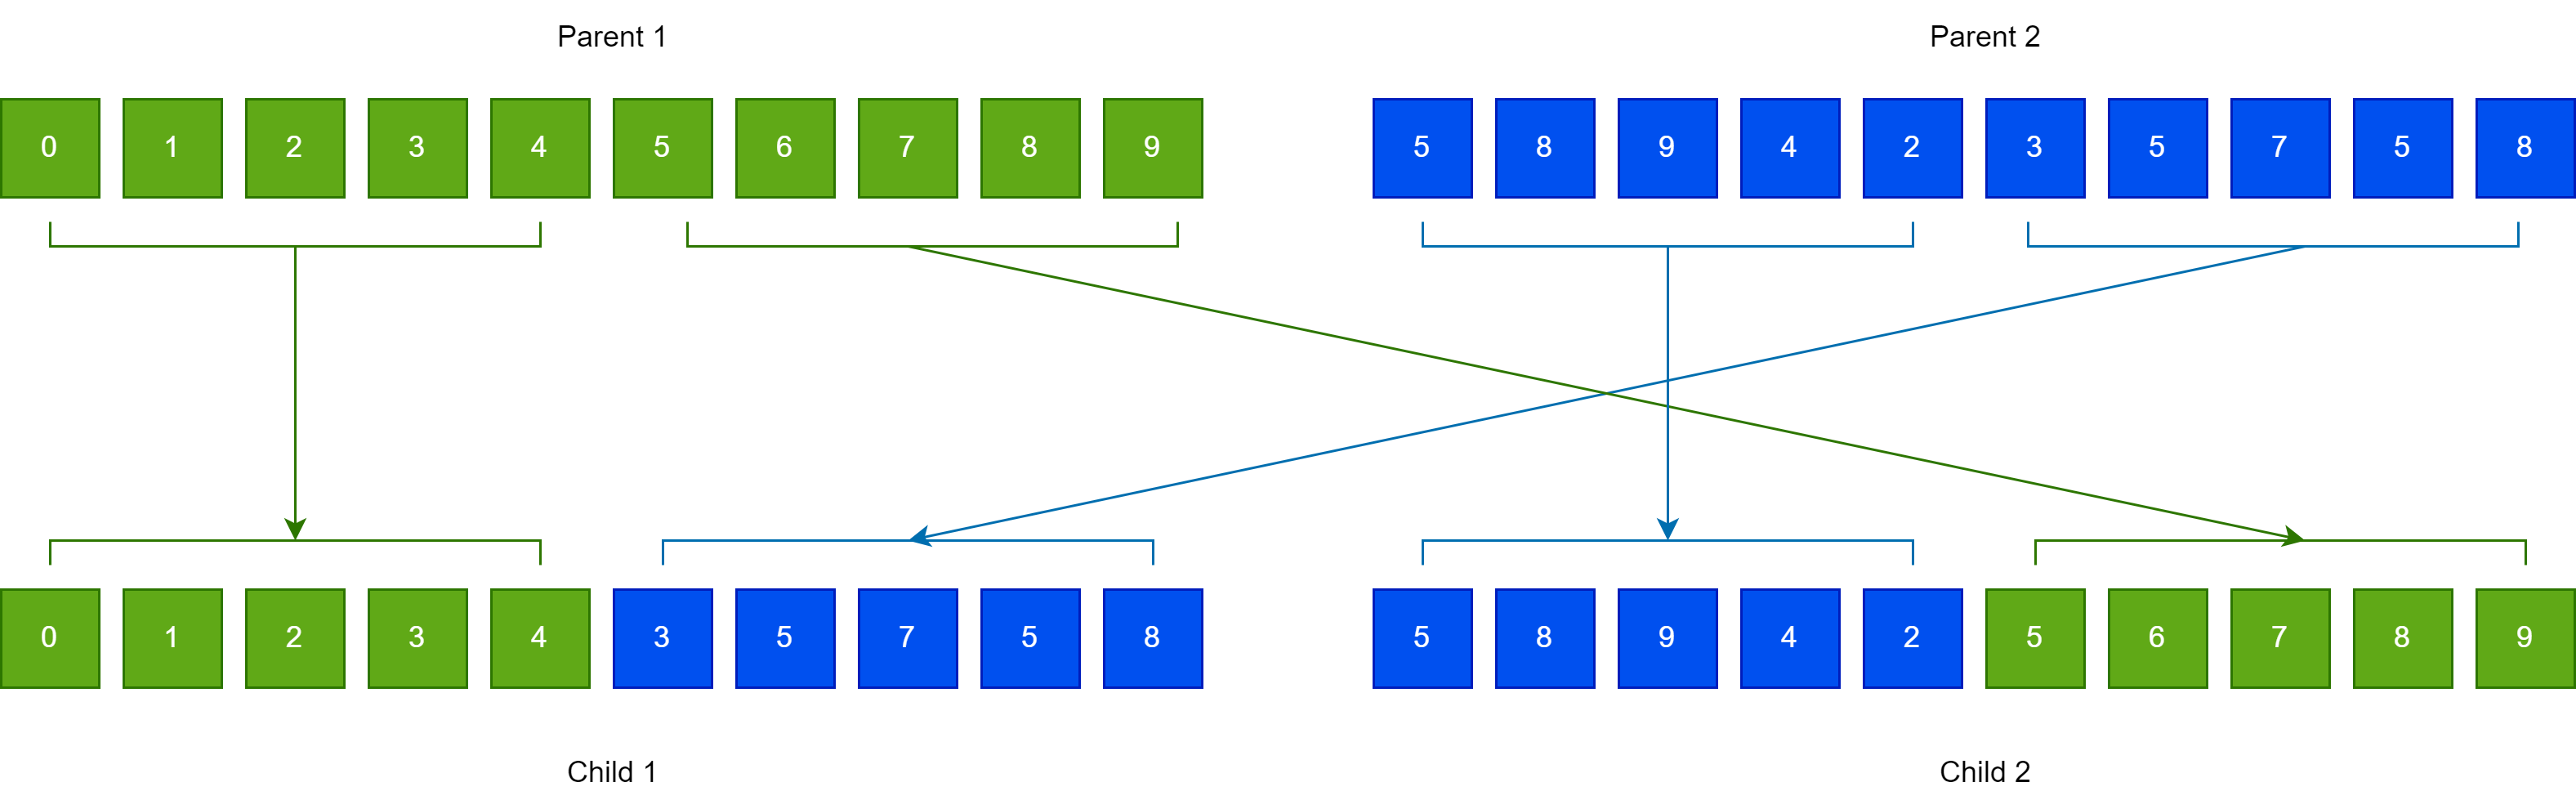
\includegraphics[scale=0.5]{onePointCrossover}

\caption{An example of the application of the one point crossover method in
the Grammatical Evolution.\label{fig:onePoint}}

\end{figure}


\subsection{Constructed neural networks \label{subsec:Constructed-neural-networks}}

Another method used in the conducted experiments is the neural network
construction method \citep{nnc}. This method can discover the optimal
architecture of artificial neural networks as well as an estimation
for the parameters of the network by using the Grammatical Evolution
technique. This method has been applied in a series of problems, such
as problems presented in chemistry \citep{nnc_amide1}, education
problems \citep{nnc_student}, autism screening \citep{nnc_autism}
etc. The BNF grammar incorporated in the neural construction procedure
is depicted in Figure \ref{fig:nncGrammar}. This grammar can produce
artificial neural networks in the following form:

\begin{equation}
N\left(\overrightarrow{x},\overrightarrow{w}\right)=\sum_{i=1}^{H}w_{(d+2)i-(d+1)}\sigma\left(\sum_{j=1}^{d}x_{j}w_{(d+2)i-(d+1)+j}+w_{(d+2)i}\right)\label{eq:nn}
\end{equation}
The value $H$ denotes the number of processing units (weights) of
the neural network. Also, the function $\sigma(x)$ stands for the
sigmoid function. Following the previous equation, it is deducted
that the total number of parameters for this network are computed
as follows:
\begin{equation}
n=\left(d+2\right)H
\end{equation}
As an example consider the following neural network:
\begin{equation}
N(x)=1.9\mbox{sig}\left(10.5x_{1}+3.2x_{3}+1.4\right)+2.1\mbox{sig}\left(2.2x_{2}-3.3x_{3}+3.2\right)
\end{equation}
This expression represents a neural network used in a problem with
3 inputs $\left(x_{1},x_{2},x_{3}\right).$The number of processing
nodes is $H=2$. This neural network is outlined graphically in Figure
\ref{fig:nnExample}.

\begin{figure}[H]
\begin{lyxcode}
S:=\textless Sigval\textgreater ~~~~~~~~~~~~~~~~~~~~~~~~~~(0)

\textless Sigval\textgreater ::=\textless Node\textgreater ~~~~~~~~~~~~~~~~~~~~(0)

~~~~~~~~~~~\textbar ~\textless Node\textgreater ~+~\textless Sigval\textgreater ~~~~~~~(1)

\textless Node\textgreater ::=\textless Number\textgreater{*}sig(\textless Sum\textgreater +\textless Number\textgreater )~(0)

\textless Sum\textgreater ::=~\textless Number\textgreater{*}\textless Xlist\textgreater ~~~~~~~~~~~~(0)

~~~~~~~~~~~\textbar ~~~~\textless Sum\textgreater +\textless Sum\textgreater ~~~~~~~~~~~(1)

\textless Xlist\textgreater ::=~x1~~~~~~~~(0)

~~~~~~~~~~~~~\textbar ~~~~x2~~(1)

~~~~~~~~~~~~~..............

~~~~~~~~~~~~~\textbar ~~~~xd~~(d-1)

\textless Number\textgreater ::=~(\textless Dlist\textgreater .\textless Dlist\textgreater )~~~~~~~~(0)

~~~~~~~~~~~~~\textbar ~~~~(-\textless Dlist\textgreater .\textless Dlist\textgreater )~(1)

\textless Dlist\textgreater ::=~\textless Digit\textgreater ~~~~~~~~~~~~(0)

~~~~~~~~~~~~~\textbar ~\textless Digit\textgreater\textless Dlist\textgreater ~(1)

\textless Digit\textgreater ::=~0~~~~~~(0)

~~~~~~~~~~~~~\textbar ~~1~(1)

~~~~~~~~~~~~~...........

~~~~~~~~~~~~~\textbar ~~9~(9)
\end{lyxcode}
\caption{The proposed grammar for the construction of artificial neural networks
through Grammatical Evolution.\label{fig:nncGrammar}}
\end{figure}
\begin{figure}[H]
\begin{centering}
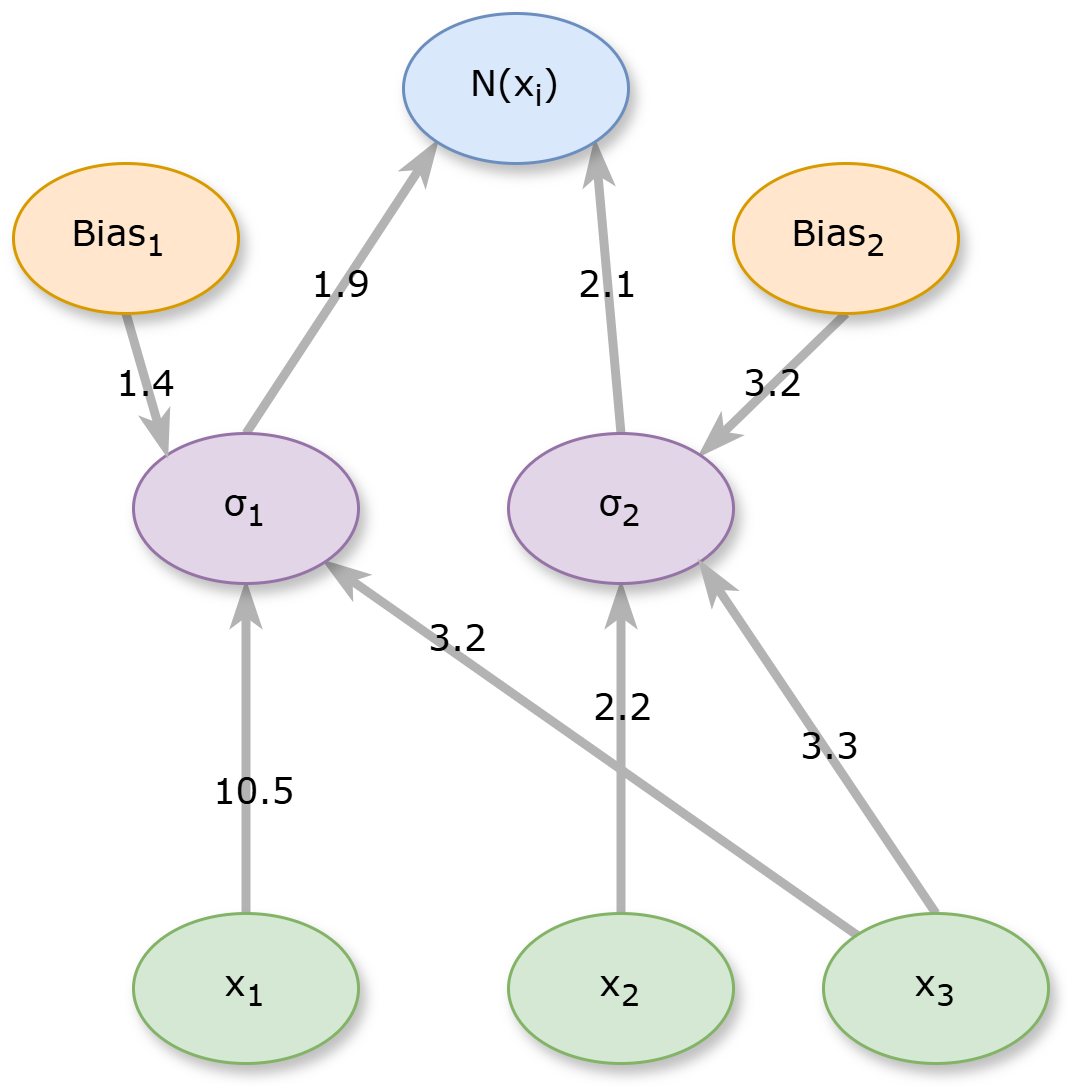
\includegraphics[scale=0.75]{/home/sheridan/Desktop/ERGASIES/GlobalOptimus/doc/NNC_GA/example_diagram}
\par\end{centering}
\caption{An example of a produced neural network.\label{fig:nnExample}}
\end{figure}
The steps of the method used to construct artificial neural networks
are shown below:
\begin{itemize}
\item \textbf{Step 1 - Initialization step}.
\begin{enumerate}
\item \textbf{Define} as $N_{c}$ the number of chromosomes in the genetic
population and as $N_{g}$ the total number of allowed generations.
\item \textbf{Set} as $p_{s}$ the used selection rate and as $p_{m}$ the
used mutation rate.
\item \textbf{Initialize} the chromosomes $c_{i},\ i=1,\ldots,N_{c}$. Each
chromosome is considered as a set of randomly selected positive integers.
\item \textbf{Set} $k=0$, as the generation counter.
\end{enumerate}
\item \textbf{Step 2 - Fitness calculation step}.
\begin{enumerate}
\item \textbf{For} $i=1,\ldots,N_{c}$ \textbf{do}
\begin{enumerate}
\item \textbf{Obtain} the chromosome $c_{i}$
\item \textbf{Create} the corresponding neural network $N_{i}\left(\overrightarrow{x},\overrightarrow{w}\right)$
for this chromosome using the grammar of Figure \ref{fig:nncGrammar}.
\item \textbf{Calculate} the associated fitness value $f_{i}$ as the training
error of network $N_{i}\left(\overrightarrow{x},\overrightarrow{w}\right)$
defined as:
\[
f_{i}=\sum_{j=1}^{M}\left(N_{i}\left(\overrightarrow{x_{j}},\overrightarrow{w}\right)-y_{j}\right)^{2}
\]
\end{enumerate}
\item \textbf{End For}
\end{enumerate}
\item \textbf{Step 3 - Application of genetic operations}. Apply the same
genetic operations as in the algorithm of subsection \ref{subsec:The-rule-production}.
\item \textbf{Step 4 - Termination check step}.
\begin{enumerate}
\item \textbf{Set} $k=k+1$
\item \textbf{Terminate} if $k\ge N_{g}$
\item \textbf{Go to} fitness calculation step.
\end{enumerate}
\end{itemize}

\subsection{The feature construction method\label{subsec:The-feature-construction}}

Another technique, based on Grammatical Evolution, used on the conducted
experiments is the Feature Construction technique, initially described
in the work of Gavrilis et al \citep{fc1}. This technique produces
artificial features from the original ones, using non linear mappings
produced by the Grammatical Evolution procedure. The BNF grammar used
for this technique is outlined in Figure \ref{fig:fcGrammar}.

\begin{figure}[H]
\caption{The grammar used in Feature Construction method.\label{fig:fcGrammar}}

\begin{lyxcode}
S::=\textless expr\textgreater ~~~(0)~

\textless expr\textgreater ~::=~~(\textless expr\textgreater ~\textless op\textgreater ~\textless expr\textgreater )~~~~~~~~~~~~~~~

~~~~~~~~~~~\textbar ~\textless func\textgreater ~(~\textless expr\textgreater ~)~~~~~~~~~~~~~~~~~

~~~~~~~~~~~\textbar\textless term\textgreater ~~~~~~~~~~~~~

\textless op\textgreater ~::=~~~~~+~~~~~~~~~~~~~~~~~~~

~~~~~~~~~~~\textbar ~-~~~~~~~~~~~~~~~~~~~

~~~~~~~~~~~\textbar ~{*}~~~~~~~~~~~~~~~~~~~

~~~~~~~~~~~\textbar ~/~~~~~~

\textless func\textgreater ~::=~~~sin~~~~~~~~~~~~~~~

~~~~~~~~~~~\textbar ~cos~~~~~~~~~~~~~~~

~~~~~~~~~~~\textbar exp~~~~~~~~~~~~~~~~

~~~~~~~~~~~\textbar log~~~

\textless term\textgreater ::=\textless xlist\textgreater ~~~~~~~~~~~~~~~~~~~~~~~~~~~~~~~~~~~~~~

~~~~~~~~~~~\textbar\textless dlist\textgreater .\textless dlist\textgreater ~

\textless xlist\textgreater ::=x1~~~~~~~~~~~~~~~~~~

~~~~~~~~~~~\textbar ~x2~~~~~~~~~~~~~~~

~~~~~~~~~~~………~~~~~~~~~~~~~

~~~~~~~~~~~\textbar ~xd~

\textless dlist\textgreater ::=\textless digit\textgreater ~~~~~~~~~~~~~~~~~~~~~~~~~~~~~~~~~~~

~~~~~~~~~~~\textbar ~\textless digit\textgreater\textless digit\textgreater ~~~~~~~~~~~~

~~~~~~~~~~~\textbar ~\textless digit\textgreater\textless digit\textgreater\textless digit\textgreater ~~~~~

\textless digit\textgreater ~~::=~0~\textbar ~1~\textbar ~2~\textbar ~3\textbar ~4\textbar ~5\textbar ~6\textbar ~7\textbar ~8\textbar ~9~
\end{lyxcode}
\end{figure}
The produced features are evaluated by Radial Basis Function (RBF)
networks \citep{rbf1,rbf2} due to the speed of their associated training
procedure. The steps of the feature construction technique have as
follows:
\begin{enumerate}
\item \textbf{Initialization step}.
\begin{enumerate}
\item \textbf{Set} the parameters of the method: $N_{c}$ the number of
chromosomes, $N_{g}$ the maximum number of allowed generations, $p_{s}$
the selection rate and $p_{m}$ the mutation rate. 
\item \textbf{Initialize} the $N_{c}$ chromosomes as sets of random integers.
\item \textbf{Set} as $N_{f}$ the number of constructed features.
\item \textbf{Set} $k=0$, the generation counter.
\end{enumerate}
\item \textbf{Fitness calculation step}.
\begin{enumerate}
\item \textbf{For} $i=1,\ldots,N_{c}$ \textbf{do}
\begin{enumerate}
\item \textbf{Produce} $N_{f}$ artificial features $y_{1},y_{2},\ldots,y_{N_{f}}$
for the processed chromosome $c_{i}$ using the grammar of Figure
\ref{fig:fcGrammar}.
\item \textbf{Modify} the original train set using the constructed features
$y_{1},y_{2},\ldots,y_{N_{f}}$.
\item \textbf{Apply} a machine learning model denoted as $M(x)$ to the
modified set and define as the fitness value $f_{i}$ the training
error of $M(x)$.
\end{enumerate}
\item \textbf{End For}
\end{enumerate}
\item \textbf{Genetic operations step}. Apply the same genetic operations
as in the algorithm of subsection \ref{subsec:The-rule-production}.
\item \textbf{Termination check step}.
\begin{enumerate}
\item \textbf{Set} $k=k+1$
\item \textbf{Terminate} when $k\ge N_{g}$
\item \textbf{Go to} fitness calculation step.
\end{enumerate}
\end{enumerate}

\section{Experimental results\label{sec:Results}}

The measurements from the years 2004, 2010 and 2012 was uses as test
cases in the experimental results. For the neural network construction
technique the freely available software NNC \citep{nnc_softx} was
incorporated. The feature construction was performed by using the
QFC software \citep{qfc}, that was also freely available. Furthermore,
the WEKA programming tool \citep{weka_main} was also utilized in
the conducted experiments. The validation of the experiments was performed
using the ten - fold cross validation technique and all experiments
were conducted on a machine running Debian Linux with 128GB of RAM.
The average regression error on the test set was measured, using the
following equation:
\begin{equation}
E_{R}\left(M\left(\overrightarrow{x}\right)\right)=\frac{\sum_{i=1}^{N}\left(N\left(\overrightarrow{x_{i}}\right)-y_{i}\right)^{2}}{N}
\end{equation}
Here the test set $T$ is defined as the set $T=\left(x_{i},y_{i}\right),\ i=1,\ldots,N$
and the equation $M\left(\overrightarrow{x}\right)$ denotes the application
of the machine learning $M(x)$ on the input pattern $\overrightarrow{x}$.
The values for the experimental parameters are outlined in Table \ref{tab:settings}.
The parameters used in the individual Genetic Algorithms have been
successfully used in the past in a multitude of research works and
furthermore constitute a compromise between the speed and performance
of the algorithms used in the present work.

\begin{table}[H]
\caption{The values used for the experimental parameters.\label{tab:settings}}

\centering{}%
\begin{tabular}{|c|c|c|}
\hline 
PARAMETER & MEANING & VALUE\tabularnewline
\hline 
\hline 
$N_{c}$ & Chromosomes & 500\tabularnewline
\hline 
$N_{g}$ & Maximum number of generations & 200\tabularnewline
\hline 
$p_{s}$ & Selection rate & 0.10\tabularnewline
\hline 
$p_{m}$ & Mutation rate & 0.05\tabularnewline
\hline 
$N_{f}$ & Number of created features & 2\tabularnewline
\hline 
$H$ & Weights & 10\tabularnewline
\hline 
\end{tabular}
\end{table}
 Also, The following notation is used in the experimental table:
\begin{enumerate}
\item The column year denotes the recording year for the earthquakes.
\item The column $D_{c}$ denotes the critical distance, expressed as mile,
used in the pre - processing of the earthquake data.
\item The column LSTM denotes the incorporation of the Long short - term
memory (LSTM) neural network \citep{lstm} as implemented in the PyTorch
programming library \citep{pytorch}. 
\item The column SVM stands for the usage of the Support Vector Machines
\citep{svm} as coded in the LibSvm library \citep{libsvm}.
\item The column MLP(BP) denotes the incorporation of the Back Propagation
algorithm \citep{bpnn1,bpnn2} in the training of a neural network
with $H=10$ processing nodes.
\item The column MLP(RPROP) represents the usage of the RPROP method \citep{rpropnn-1,rpropnn-2}
for the training of a neural network with $H=10$ processing nodes.
\item The column MLP(BFGS) denotes the usage of the BFGS optimization procedure
\citep{powell} for the training of an artificial neural network with
$H=10$ processing nodes.
\item The column RULE denotes the incorporation of the rule construction
method, described in subsection \ref{subsec:The-rule-production}.
\item The column NNC represents the usage of the Neural Network Construction
method, provided in subsection \ref{subsec:Constructed-neural-networks}.
\item The column FC stands for the usage of the Feature Construction technique,
outlined in subsection \ref{subsec:The-feature-construction}.
\item The row AVERAGE stands for the average error for all years and critical
distances.
\end{enumerate}
\begin{table}[H]
\caption{Experimental results using a series of machine learning methods.\label{tab:expResults}}

\centering{}%
\begin{tabular}{|c|c|c|c|c|c|c|c|c|c|}
\hline 
{\footnotesize\textbf{YEAR}} & {\footnotesize\textbf{$D_{c}$}} & {\footnotesize\textbf{LSTM}} & {\footnotesize\textbf{SVM}} & {\footnotesize\textbf{MLP(BP)}} & {\footnotesize\textbf{MLP(RPROP)}} & {\footnotesize\textbf{MLP(BFGS)}} & {\footnotesize\textbf{RULE}} & {\footnotesize\textbf{NNC}} & {\footnotesize\textbf{FC}}\tabularnewline
\hline 
\hline 
{\footnotesize 2004} & {\footnotesize 10} & {\footnotesize 0.25} & {\footnotesize 0.29} & {\footnotesize 0.44} & {\footnotesize 0.24} & {\footnotesize 0.82} & {\footnotesize 0.16} & {\footnotesize 0.16} & {\footnotesize 0.17}\tabularnewline
\hline 
{\footnotesize 2004} & {\footnotesize 25} & {\footnotesize 0.23} & {\footnotesize 0.29} & {\footnotesize 0.42} & {\footnotesize 0.24} & {\footnotesize 0.98} & {\footnotesize 0.17} & {\footnotesize 0.17} & {\footnotesize 0.17}\tabularnewline
\hline 
{\footnotesize 2004} & {\footnotesize 50} & {\footnotesize 0.24} & {\footnotesize 0.29} & {\footnotesize 0.43} & {\footnotesize 0.24} & {\footnotesize 0.87} & {\footnotesize 0.17} & {\footnotesize 0.17} & {\footnotesize 0.16}\tabularnewline
\hline 
{\footnotesize 2004} & {\footnotesize 100} & {\footnotesize 0.23} & {\footnotesize 0.28} & {\footnotesize 0.35} & {\footnotesize 0.22} & {\footnotesize 0.69} & {\footnotesize 0.16} & {\footnotesize 0.16} & {\footnotesize 0.16}\tabularnewline
\hline 
{\footnotesize 2004} & {\footnotesize 500} & {\footnotesize 0.24} & {\footnotesize 0.26} & {\footnotesize 0.45} & {\footnotesize 0.27} & {\footnotesize 0.65} & {\footnotesize 0.16} & {\footnotesize 0.16} & {\footnotesize 0.16}\tabularnewline
\hline 
{\footnotesize 2010} & {\footnotesize 10} & {\footnotesize 0.24} & {\footnotesize 0.30} & {\footnotesize 0.36} & {\footnotesize 0.24} & {\footnotesize 0.74} & {\footnotesize 0.19} & {\footnotesize 0.17} & {\footnotesize 0.19}\tabularnewline
\hline 
{\footnotesize 2010} & {\footnotesize 25} & {\footnotesize 0.24} & {\footnotesize 0.30} & {\footnotesize 0.37} & {\footnotesize 0.21} & {\footnotesize 0.49} & {\footnotesize 0.19} & {\footnotesize 0.18} & {\footnotesize 0.17}\tabularnewline
\hline 
{\footnotesize 2010} & {\footnotesize 50} & {\footnotesize 0.23} & {\footnotesize 0.30} & {\footnotesize 0.39} & {\footnotesize 0.24} & {\footnotesize 0.60} & {\footnotesize 0.18} & {\footnotesize 0.17} & {\footnotesize 0.18}\tabularnewline
\hline 
{\footnotesize 2010} & {\footnotesize 100} & {\footnotesize 0.24} & {\footnotesize 0.30} & {\footnotesize 0.31} & {\footnotesize 0.27} & {\footnotesize 0.40} & {\footnotesize 0.19} & {\footnotesize 0.18} & {\footnotesize 0.19}\tabularnewline
\hline 
{\footnotesize 2010} & {\footnotesize 500} & {\footnotesize 0.25} & {\footnotesize 0.29} & {\footnotesize 0.40} & {\footnotesize 0.32} & {\footnotesize 0.51} & {\footnotesize 0.19} & {\footnotesize 0.18} & {\footnotesize 0.18}\tabularnewline
\hline 
{\footnotesize 2012} & {\footnotesize 10} & {\footnotesize 0.21} & {\footnotesize 0.28} & {\footnotesize 0.33} & {\footnotesize 0.22} & {\footnotesize 0.45} & {\footnotesize 0.18} & {\footnotesize 0.17} & {\footnotesize 0.19}\tabularnewline
\hline 
{\footnotesize 2012} & {\footnotesize 25} & {\footnotesize 0.24} & {\footnotesize 0.28} & {\footnotesize 0.33} & {\footnotesize 0.24} & {\footnotesize 0.75} & {\footnotesize 0.17} & {\footnotesize 0.17} & {\footnotesize 0.16}\tabularnewline
\hline 
{\footnotesize 2012} & {\footnotesize 50} & {\footnotesize 0.22} & {\footnotesize 0.27} & {\footnotesize 0.36} & {\footnotesize 0.23} & {\footnotesize 0.21} & {\footnotesize 0.17} & {\footnotesize 0.17} & {\footnotesize 0.16}\tabularnewline
\hline 
{\footnotesize 2012} & {\footnotesize 100} & {\footnotesize 0.23} & {\footnotesize 0.26} & {\footnotesize 0.38} & {\footnotesize 0.21} & {\footnotesize 0.57} & {\footnotesize 0.17} & {\footnotesize 0.17} & {\footnotesize 0.16}\tabularnewline
\hline 
{\footnotesize 2012} & {\footnotesize 500} & {\footnotesize 0.22} & {\footnotesize 0.25} & {\footnotesize 0.35} & {\footnotesize 0.29} & {\footnotesize 0.85} & {\footnotesize 0.17} & {\footnotesize 0.17} & {\footnotesize 0.16}\tabularnewline
\hline 
{\footnotesize\textbf{AVERAGE}} &  & {\footnotesize\textbf{0.234}} & {\footnotesize\textbf{0.283}} & {\footnotesize\textbf{0.378}} & {\footnotesize\textbf{0.245}} & {\footnotesize\textbf{0.639}} & {\footnotesize\textbf{0.175}} & {\footnotesize\textbf{0.170}} & {\footnotesize\textbf{0.171}}\tabularnewline
\hline 
\end{tabular}
\end{table}
An example of constructed features for the year 2010 is presented
below: 
\[
\begin{array}{ccc}
f_{1}(x) & = & \frac{-4}{99.35}x_{2}+\cos\left(x_{3}-877.38x_{6}+\sin\left(43.56x_{4}+x_{6}-99.35x_{2}\right)\right)\\
f_{2}(x) & = & 2x_{13}-95.2x_{2}+948.94x_{1}
\end{array}
\]

According to the data from the \ref{tab:expResults} for seismic magnitude
prediction (2004) based on neighboring earthquakes, the following
key observations are made: The grammatical evolution models (RULE,
NNC, FC) continuously exhibit the lowest regression error (0.16--0.17)
at all distances $\left(D_{c}\right)$. They are much more stable
and accurate than the other models, with an average error of 0.164.
This suggests that grammatical evolution significantly improves performance.
Among the models without grammatical evolution, LSTM and MLP-RPROP
have the best performance with an average error around 0.24 and demonstrate
decent stability at different distances. SVM has a slightly higher
average error (0.282) but is also relatively stable. MLP-BP has a
higher average error (0.418), with some improvement at greater distances
(e.g., 0.35 at 100 miles). MLP-BFGS exhibits the worst error (average
0.802) and very high variance, particularly at short distances (0.98
at 25 miles), indicating significant instability. Distance (Dc) seems
to minimally affect the error for most models (LSTM, SVM, MLP-RPROP,
and the grammatical models), suggesting robustness. The significant
exception is MLP-BFGS, which shows marked sensitivity to distance.
In summary, the grammatical evolution models (RULE, NNC, FC) are clearly
the most accurate and reliable for this prediction problem. Among
the rest, LSTM and MLP-RPROP are the best choices due to balanced
performance, while MLP-BFGS appears unsuitable due to high and unpredictable
error.

For the year 2010, the grammatical evolution models (RULE, NNC, FC)
maintain the lowest regression error (0.17--0.19) at all distances,
with NNC achieving the best average (0.176). They are more stable
than most non-evolutionary models, confirming that grammatical evolution
provides reliable predictions. Among the other models, LSTM shows
the best performance (average error 0.24) with remarkable stability
at all distances. MLP-RPROP has a slightly higher average error (0.256)
but with greater variance, particularly at long distances (0.32 at
500 miles). SVM remains stable (average 0.298) with no significant
fluctuations. MLP-BP improves at medium distances (0.31 at 100 miles)
but has a higher average error (0.366). MLP-BFGS improves compared
to 2004 (average error 0.548) but still exhibits significant variance
and high error at short distances (0.74 at 10 miles). Distance (Dc)
minimally affects most models, with the exception of MLP-BFGS and,
to a lesser extent, MLP-RPROP, which show sensitivity. Overall, the
grammatical models (especially NNC) and LSTM stand out as the most
reliable approaches for this prediction problem.

Similarly, in 2012, the grammatical evolution models (RULE, NNC, FC)
continue to maintain the lowest and most stable regression error at
all distances. NNC and FC achieve the best average error (0.17 and
0.166 respectively), with FC demonstrating remarkable stability (0.16)
at most distances. RULE has a slightly higher average (0.172). This
confirms the superiority of grammatical evolution for this problem.
Among the non-evolutionary models, LSTM stands out with the best average
error (0.224) and very good stability at different distances. MLP-RPROP
has a similar average (0.238) but greater variance, particularly at
long distances (0.29 at 500 miles). SVM improves significantly compared
to previous years (average error 0.268) and is stable. MLP-BP has
the highest error (0.35) among non-evolutionary models, with increasing
error at medium distances (0.38 at 100 miles). MLP-BFGS continues
to have the highest average error (0.566) and explosive variance,
ranging from extremely low error (0.21 at 50 miles) to very high (0.85
at 500 miles), making it unreliable. Distance (Dc) minimally affects
the grammatical models, LSTM, and SVM. MLP-BP shows sensitivity at
medium distances, while MLP-RPROP and particularly MLP-BFGS show strong
sensitivity at specific distances. Overall, for 2012, the grammatical
models (especially FC and NNC) and LSTM stand out as the most accurate
and stable approaches. MLP-BFGS remains unsuitable due to unpredictable
performance, while MLP-BP has the highest error among traditional
models. There is a general improvement in SVM and stability in LSTM
compared to previous years.

In Figure \ref{fig:2004}, the grammatical models (RULE, NNC, FC)
exhibit the lowest and most stable error (0.16--0.17) across all
distances, clearly outperforming the others. LSTM and MLP-RPROP are
the best non-evolutionary models (average error \textasciitilde 0.24),
while MLP-BFGS shows significant instability (average 0.802) with
particularly high errors at short distances.
\begin{figure}[H]
\begin{centering}
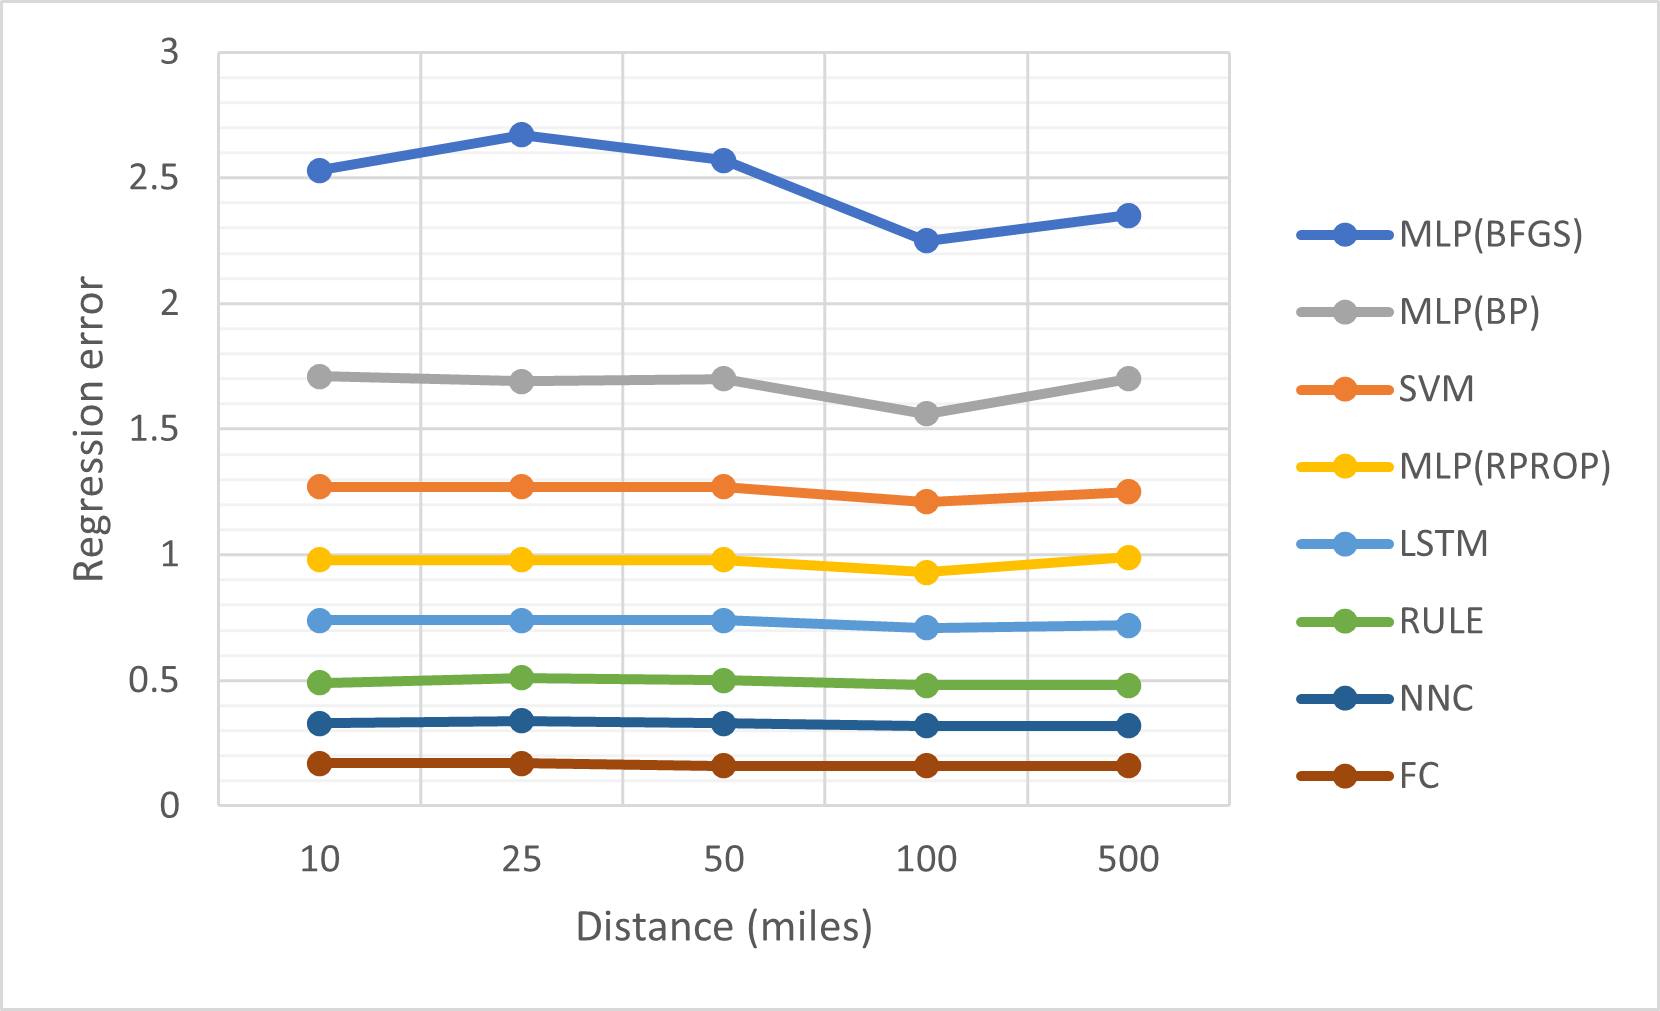
\includegraphics[scale=0.75]{2004}
\par\end{centering}
\caption{Error per point for each used method using the 2004 dataset and different
values of the critical parameter $D_{c}$\label{fig:2004}}

\end{figure}

In Figure \ref{fig:2010}, the grammatical models maintain their superiority
with an average error of 0.176--0.188, with NNC standing out. LSTM
continues to be the top non-evolutionary model (average 0.24) with
remarkable stability, while MLP-BFGS improves compared to 2004 (average
0.548) but retains significant variation, especially at short distances.

\begin{figure}[H]
\begin{centering}
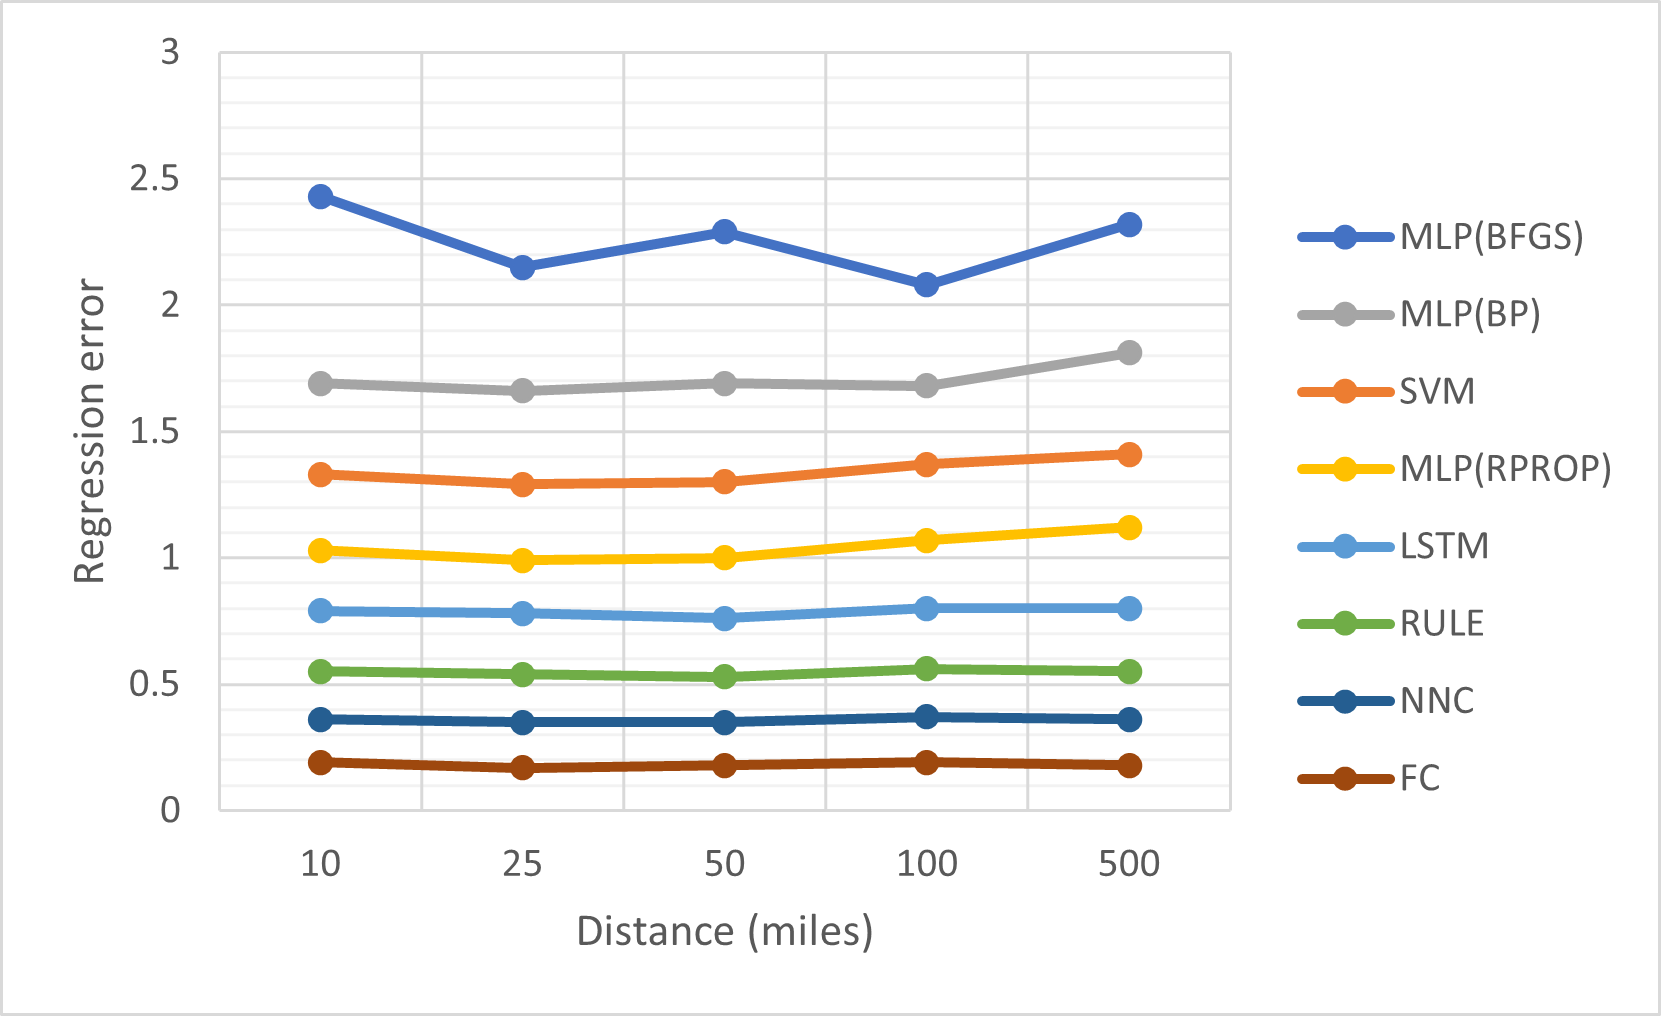
\includegraphics[scale=0.75]{2010}
\par\end{centering}
\caption{Error per point for each used method using the 2010 dataset and a
variety of values of the critical parameter $D_{c}$\label{fig:2010}}
\end{figure}
 In Figure \ref{fig:2012}, the grammatical models achieve their best
performance, with FC (average 0.166) and NNC (0.17) demonstrating
exceptional stability. LSTM remains the most reliable non-evolutionary
model (average 0.224), while MLP-BFGS shows extreme variation (from
0.21 to 0.85) despite its reduced average error (0.566).

\begin{figure}[H]
\begin{centering}
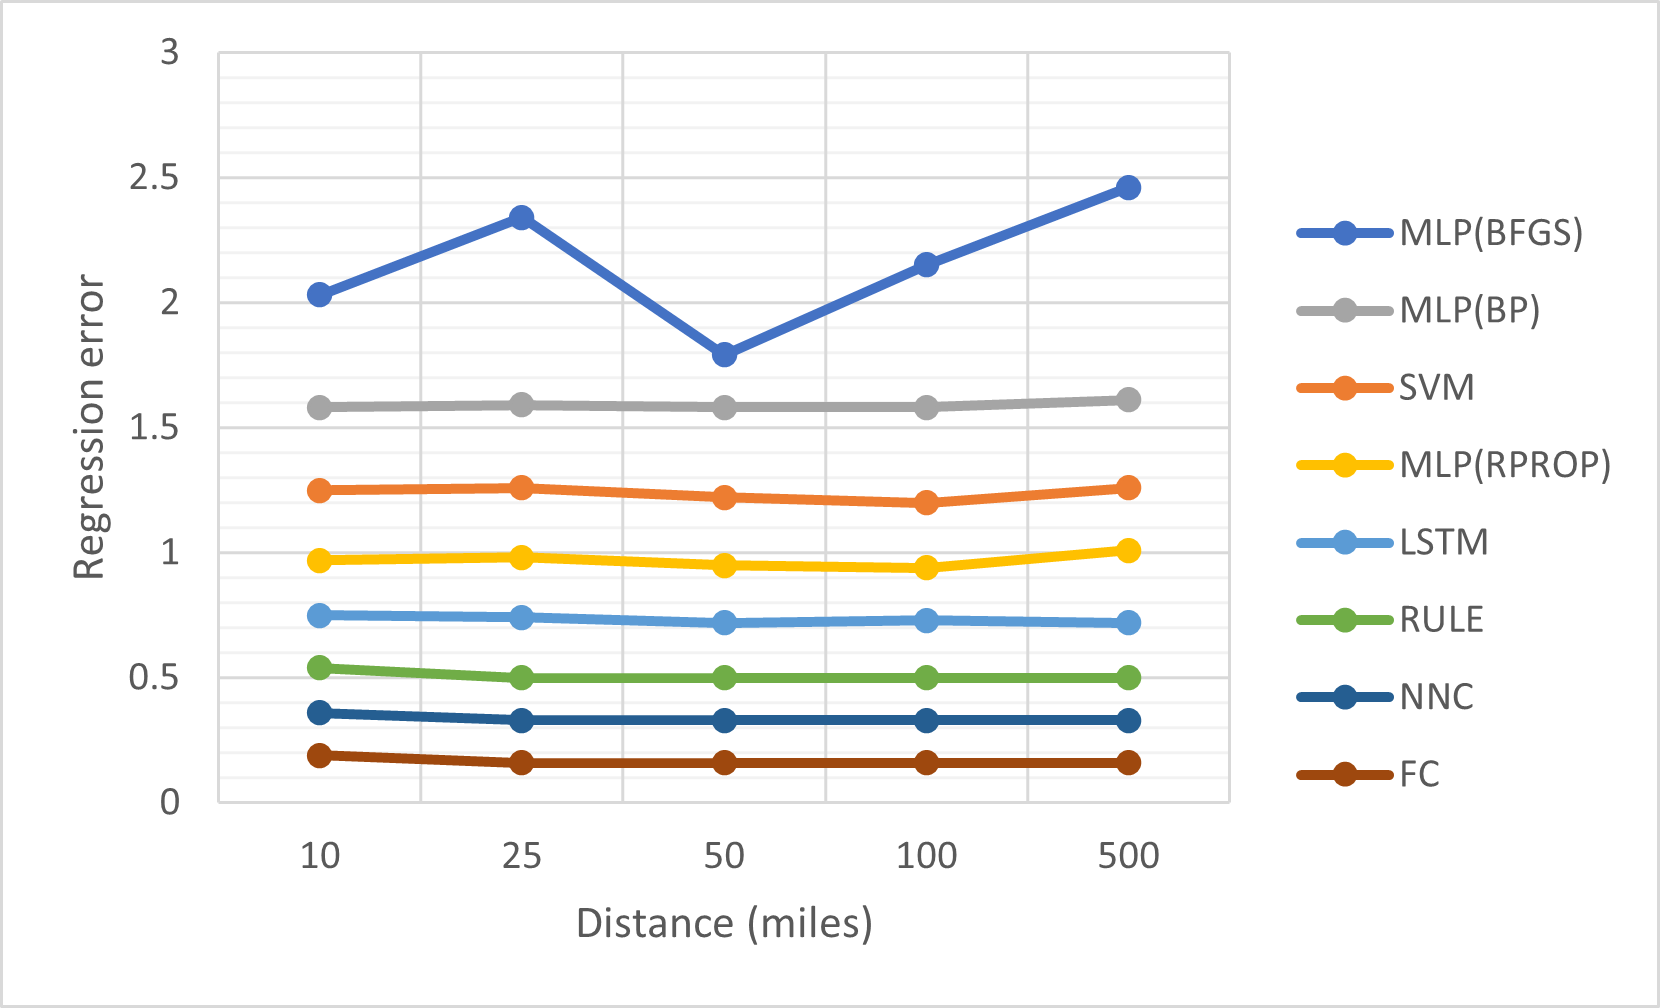
\includegraphics[scale=0.75]{2012}
\par\end{centering}
\caption{Error per point the machine learning methods using the 2012 and a
series of values for the critical parameter $D_{c}$\label{fig:2012}}
\end{figure}
According to the results of the Friedman test \ref{fig:friedman},
where the overall difference between the models is extremely statistically
significant (p=4.51e-18 \textless{} 0.0001, critical value=4.2863,
critical difference=3.834), the following key stratifications are
observed: The models with Grammatical Evolution (RULE, NNC, FC) show
homogeneous performance (p=ns among them) but are significantly better
(p={*}{*}{*}{*}) than MLP(BP) and MLP(BFGS). They also significantly
outperform SVM (p={*}{*}{*}{*} for NNC/FC, p={*}{*}{*} for RULE).
LSTM (without Grammar-Based Evolution) does not differ significantly
either from the models with Grammar-Based Evolution (p=ns) or from
SVM, MLP(BP), and MLP(RPROP) (p=ns), with the only significant difference
being against MLP(BFGS) (p={*}{*}). MLP(RPROP) (without Grammar-Based
Evolution) does not differ from RULE (p=ns) but shows significantly
higher error than NNC/FC (p={*}) and MLP(BFGS) (p={*}). MLP(BFGS)
(without Grammar-Based Evolution) is the least reliable model, with
significantly worse performance (p={*}{*}{*}) compared to all models
with Grammar-Based Evolution and significantly worse than LSTM (p={*}{*})
and MLP(RPROP) (p={*}).
\begin{figure}[H]
\begin{centering}
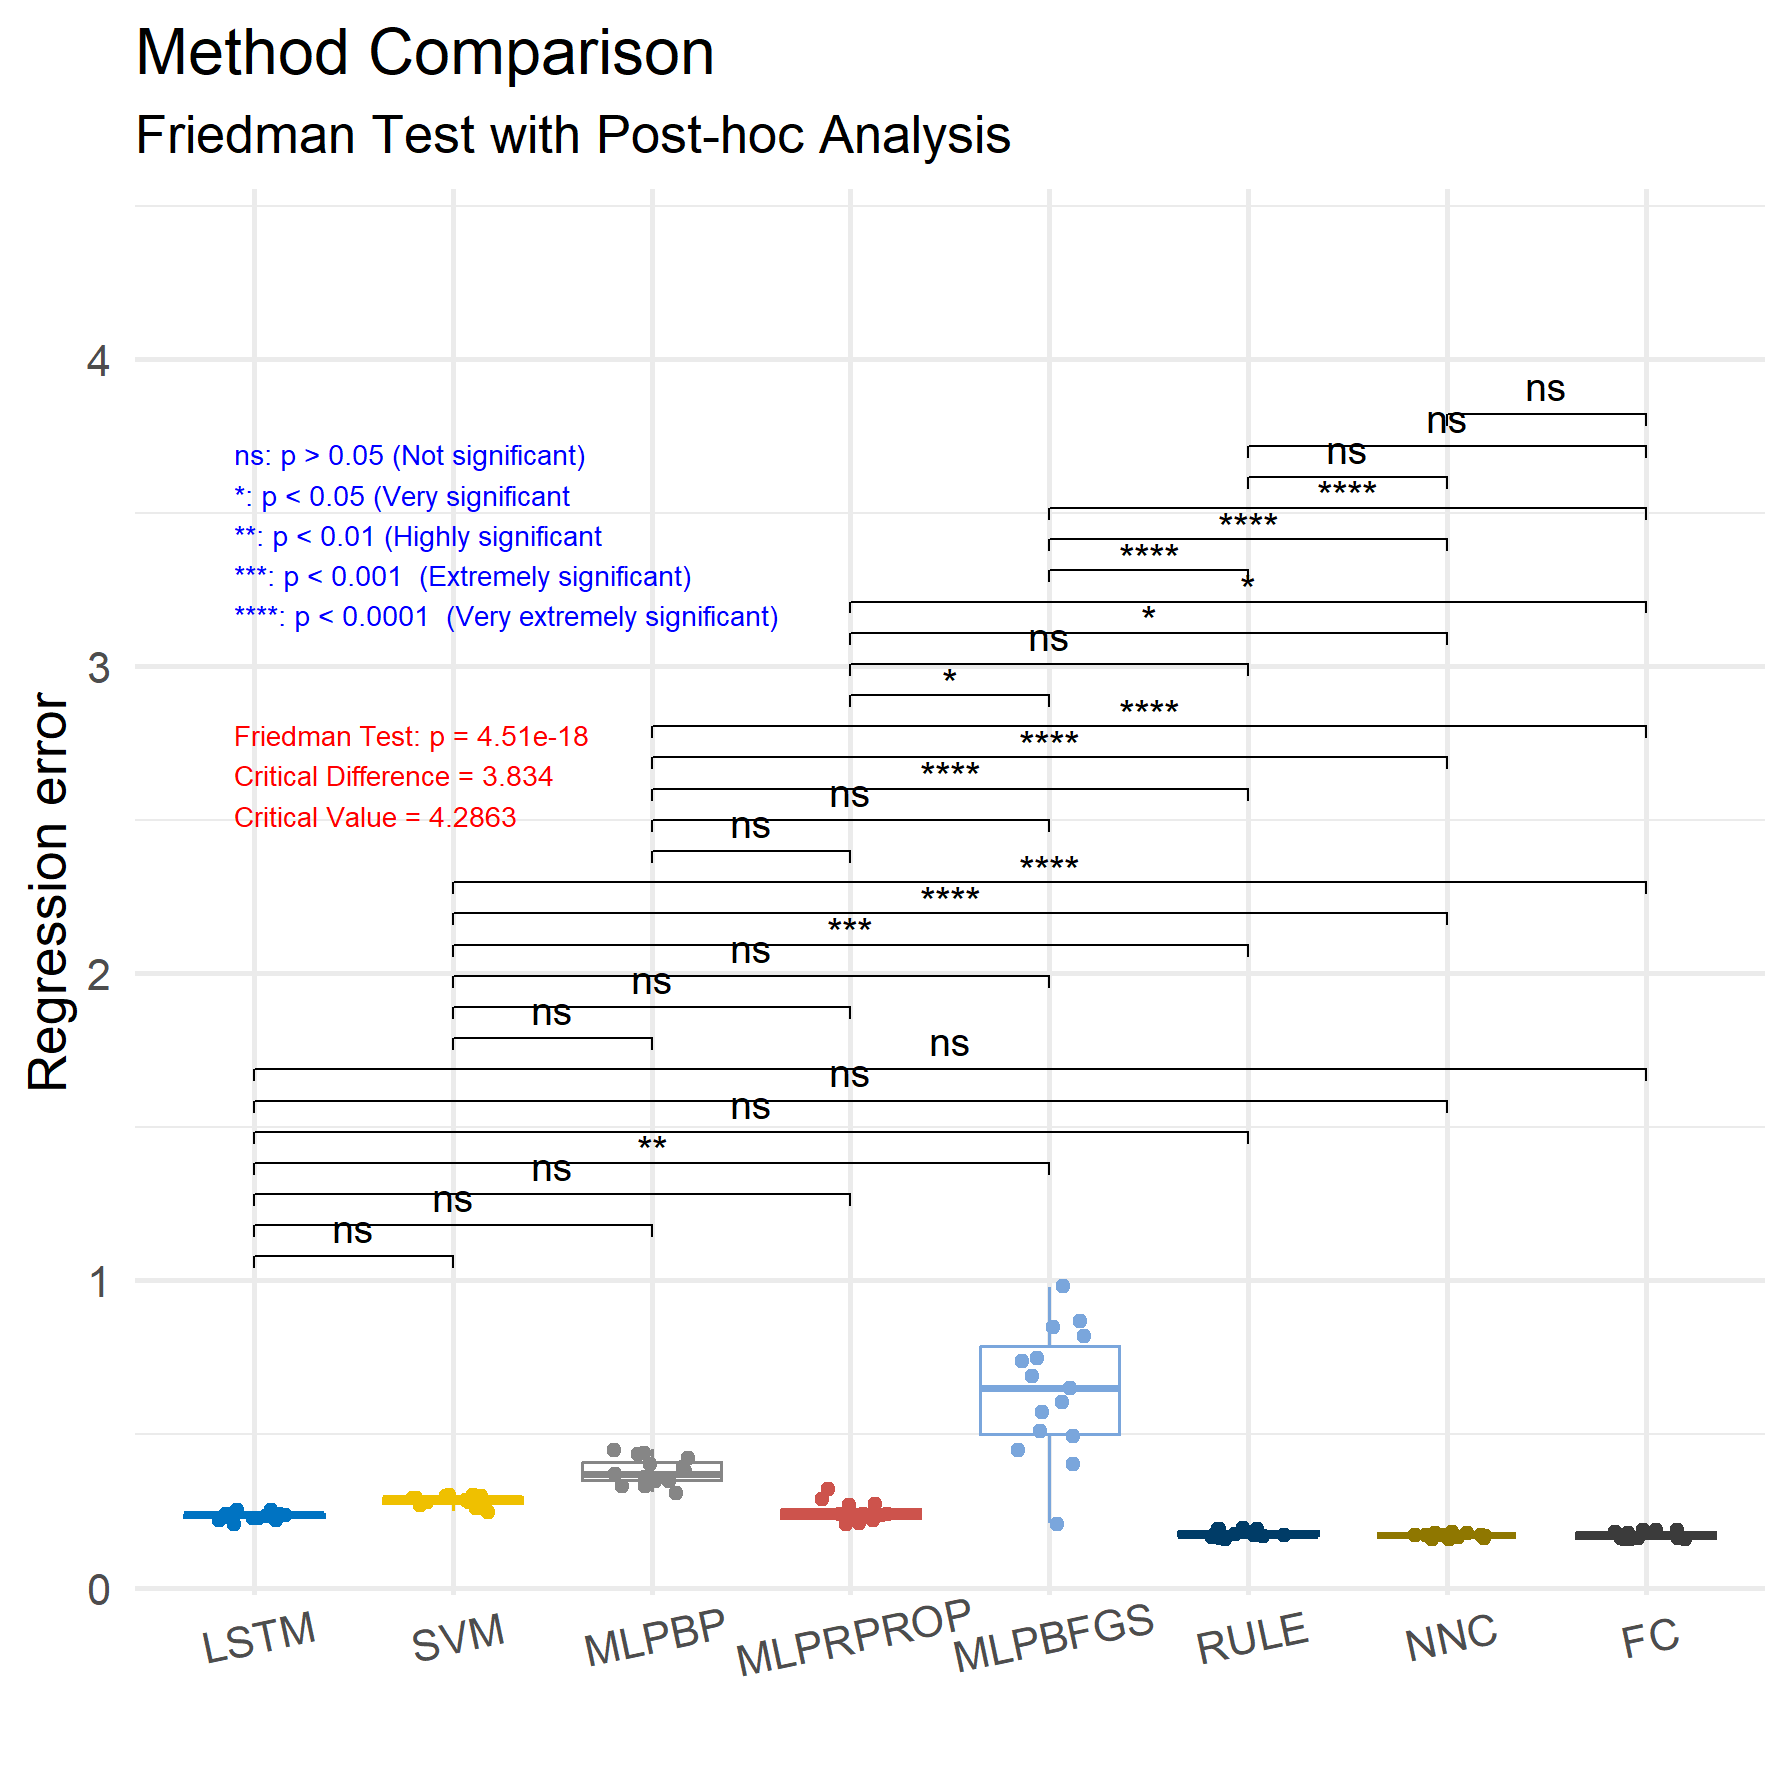
\includegraphics[scale=0.5]{stat3}
\par\end{centering}
\caption{Method comparison using Friedman test.\label{fig:friedman}}

\end{figure}

In Figures \ref{fig:graphYear} and \ref{fig:distanceError}, the
prediction error analysis results for different machine learning models
are presented. We observe significant differences between the two
model categories. The analysis reveals that models without grammatical
evolution exhibit greater variability in prediction errors. Notably,
one of these models shows particularly high errors at certain distances,
indicating a lack of stability. In contrast, the most effective model
in this category maintains relatively low errors across all distances.
The methods with grammatical evolution demonstrate remarkable stability
and lower errors. The three models in this category show similar and
consistent performance, with minimal variations across different distances
and years. The effect of distance is clearly visible in models without
grammatical evolution, where errors vary significantly. Conversely,
in models with grammatical evolution, distance does not appear to
significantly affect prediction accuracy. Temporally, while models
without grammatical evolution show some improvement over time, models
with grammatical evolution maintain stable performance throughout
the study period. Overall, the results support the superiority of
methods with grammatical evolution, which demonstrate greater reliability
and stability under various conditions. This ability to effectively
handle data variations makes them an ideal choice for applications
requiring accurate and stable predictions.

\begin{figure}[H]
\begin{centering}
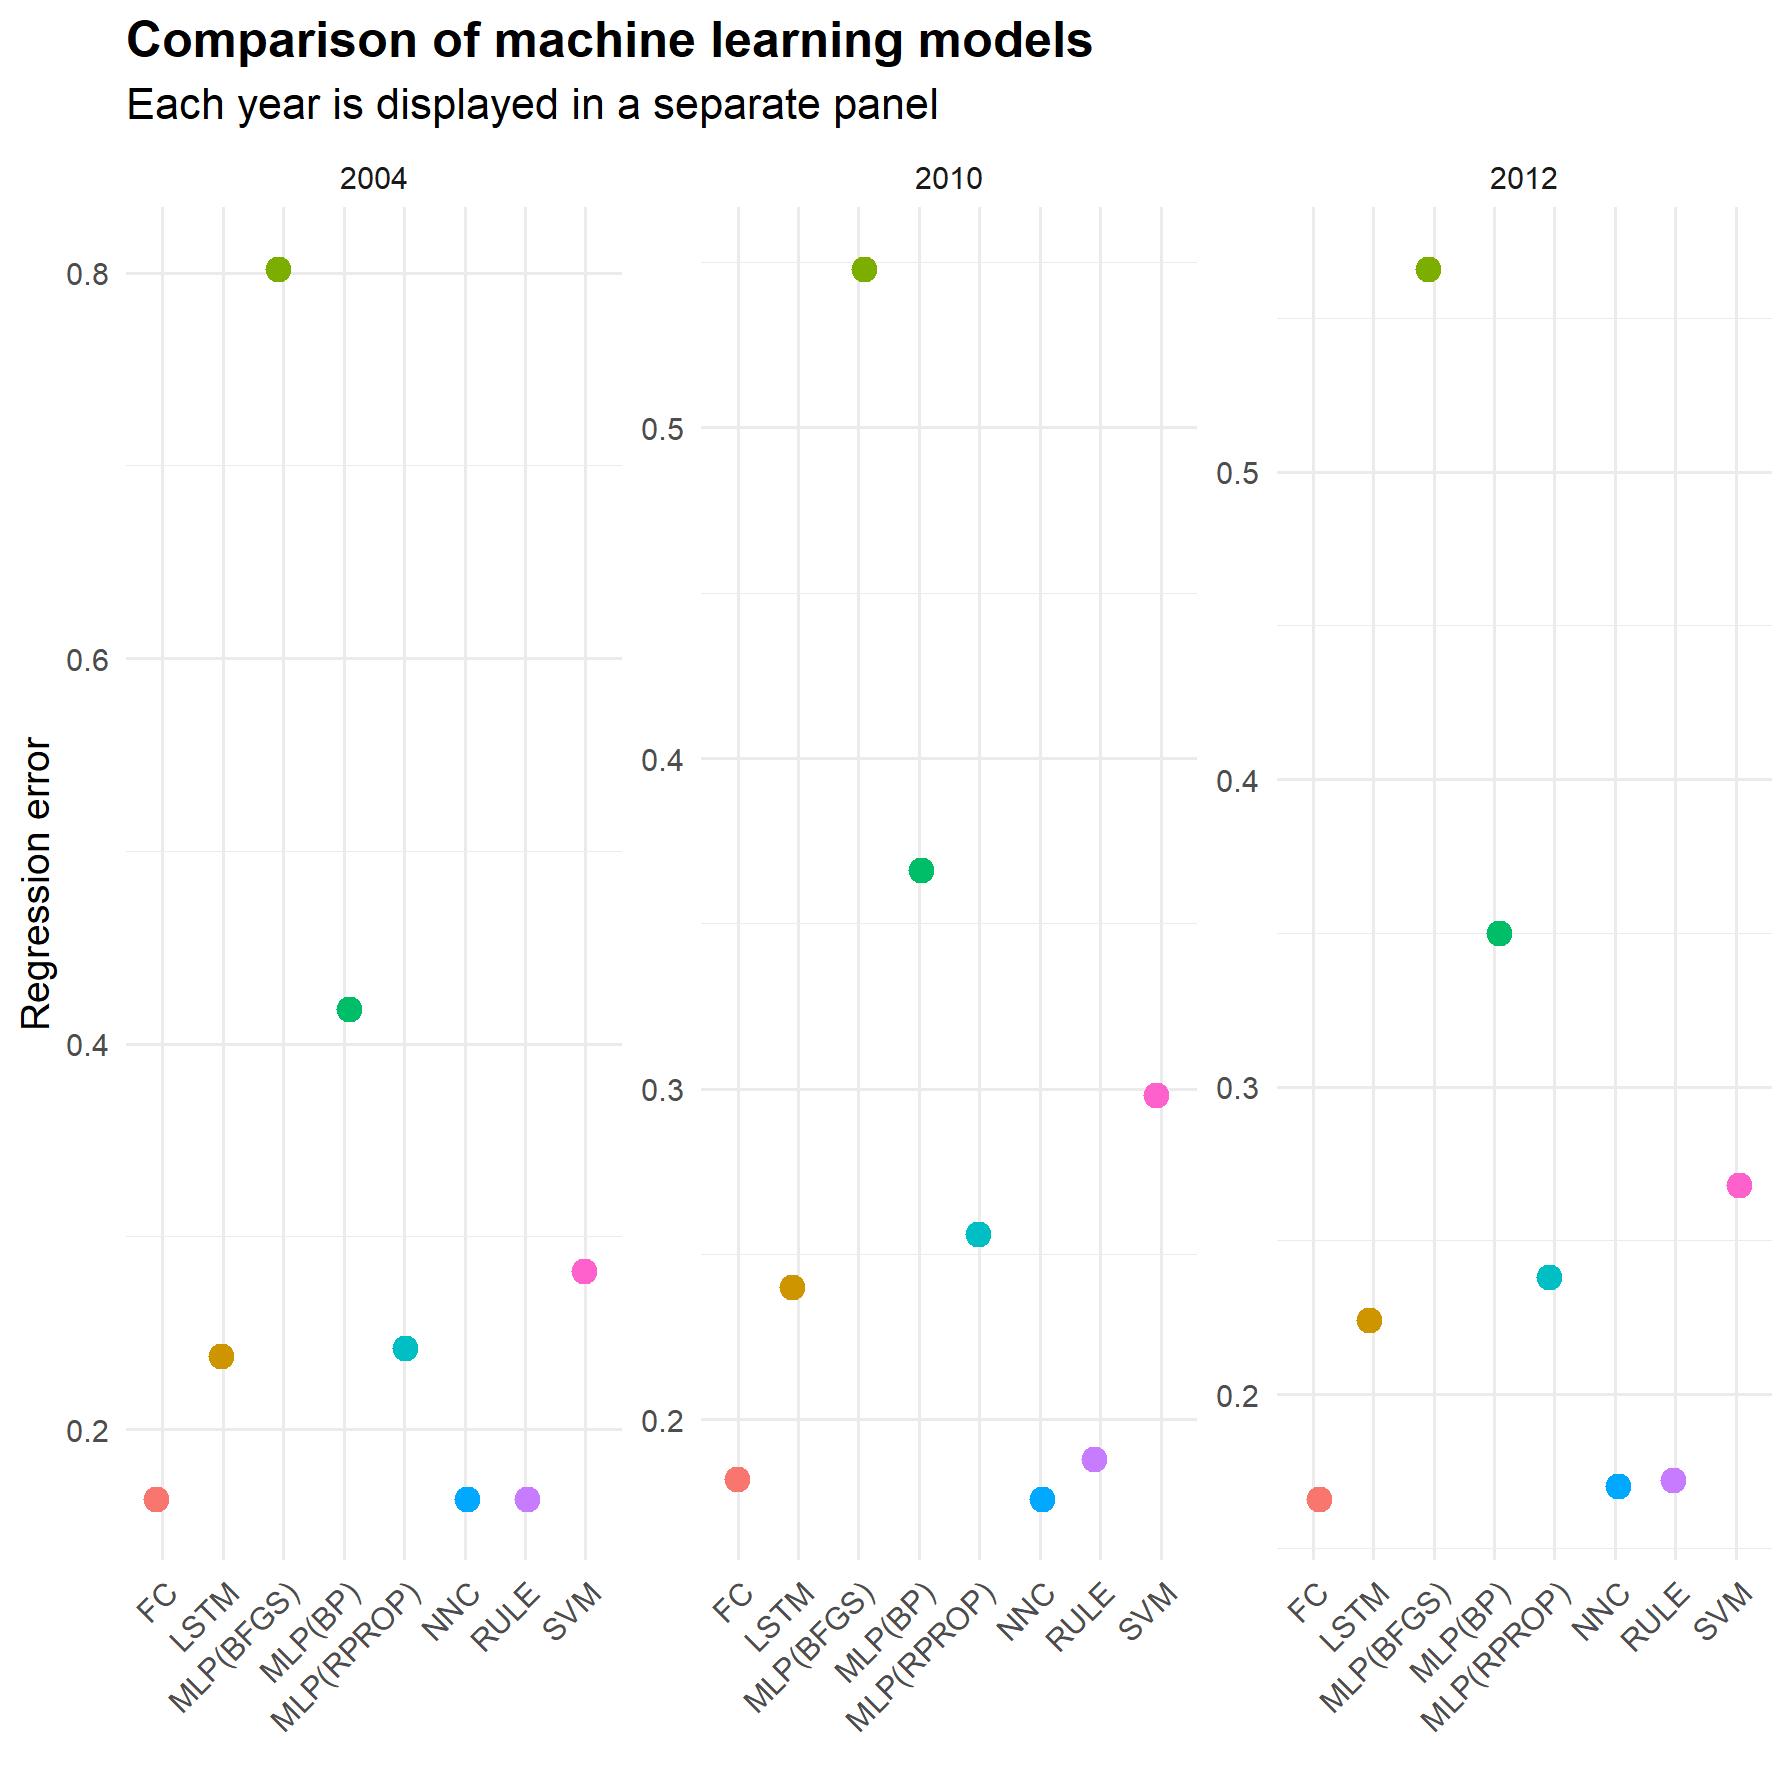
\includegraphics[scale=0.5]{stat1}
\par\end{centering}
\caption{Comparison of machine learning models for every year participated
in the experiments.\label{fig:graphYear}}

\end{figure}
\begin{figure}[H]
\begin{centering}
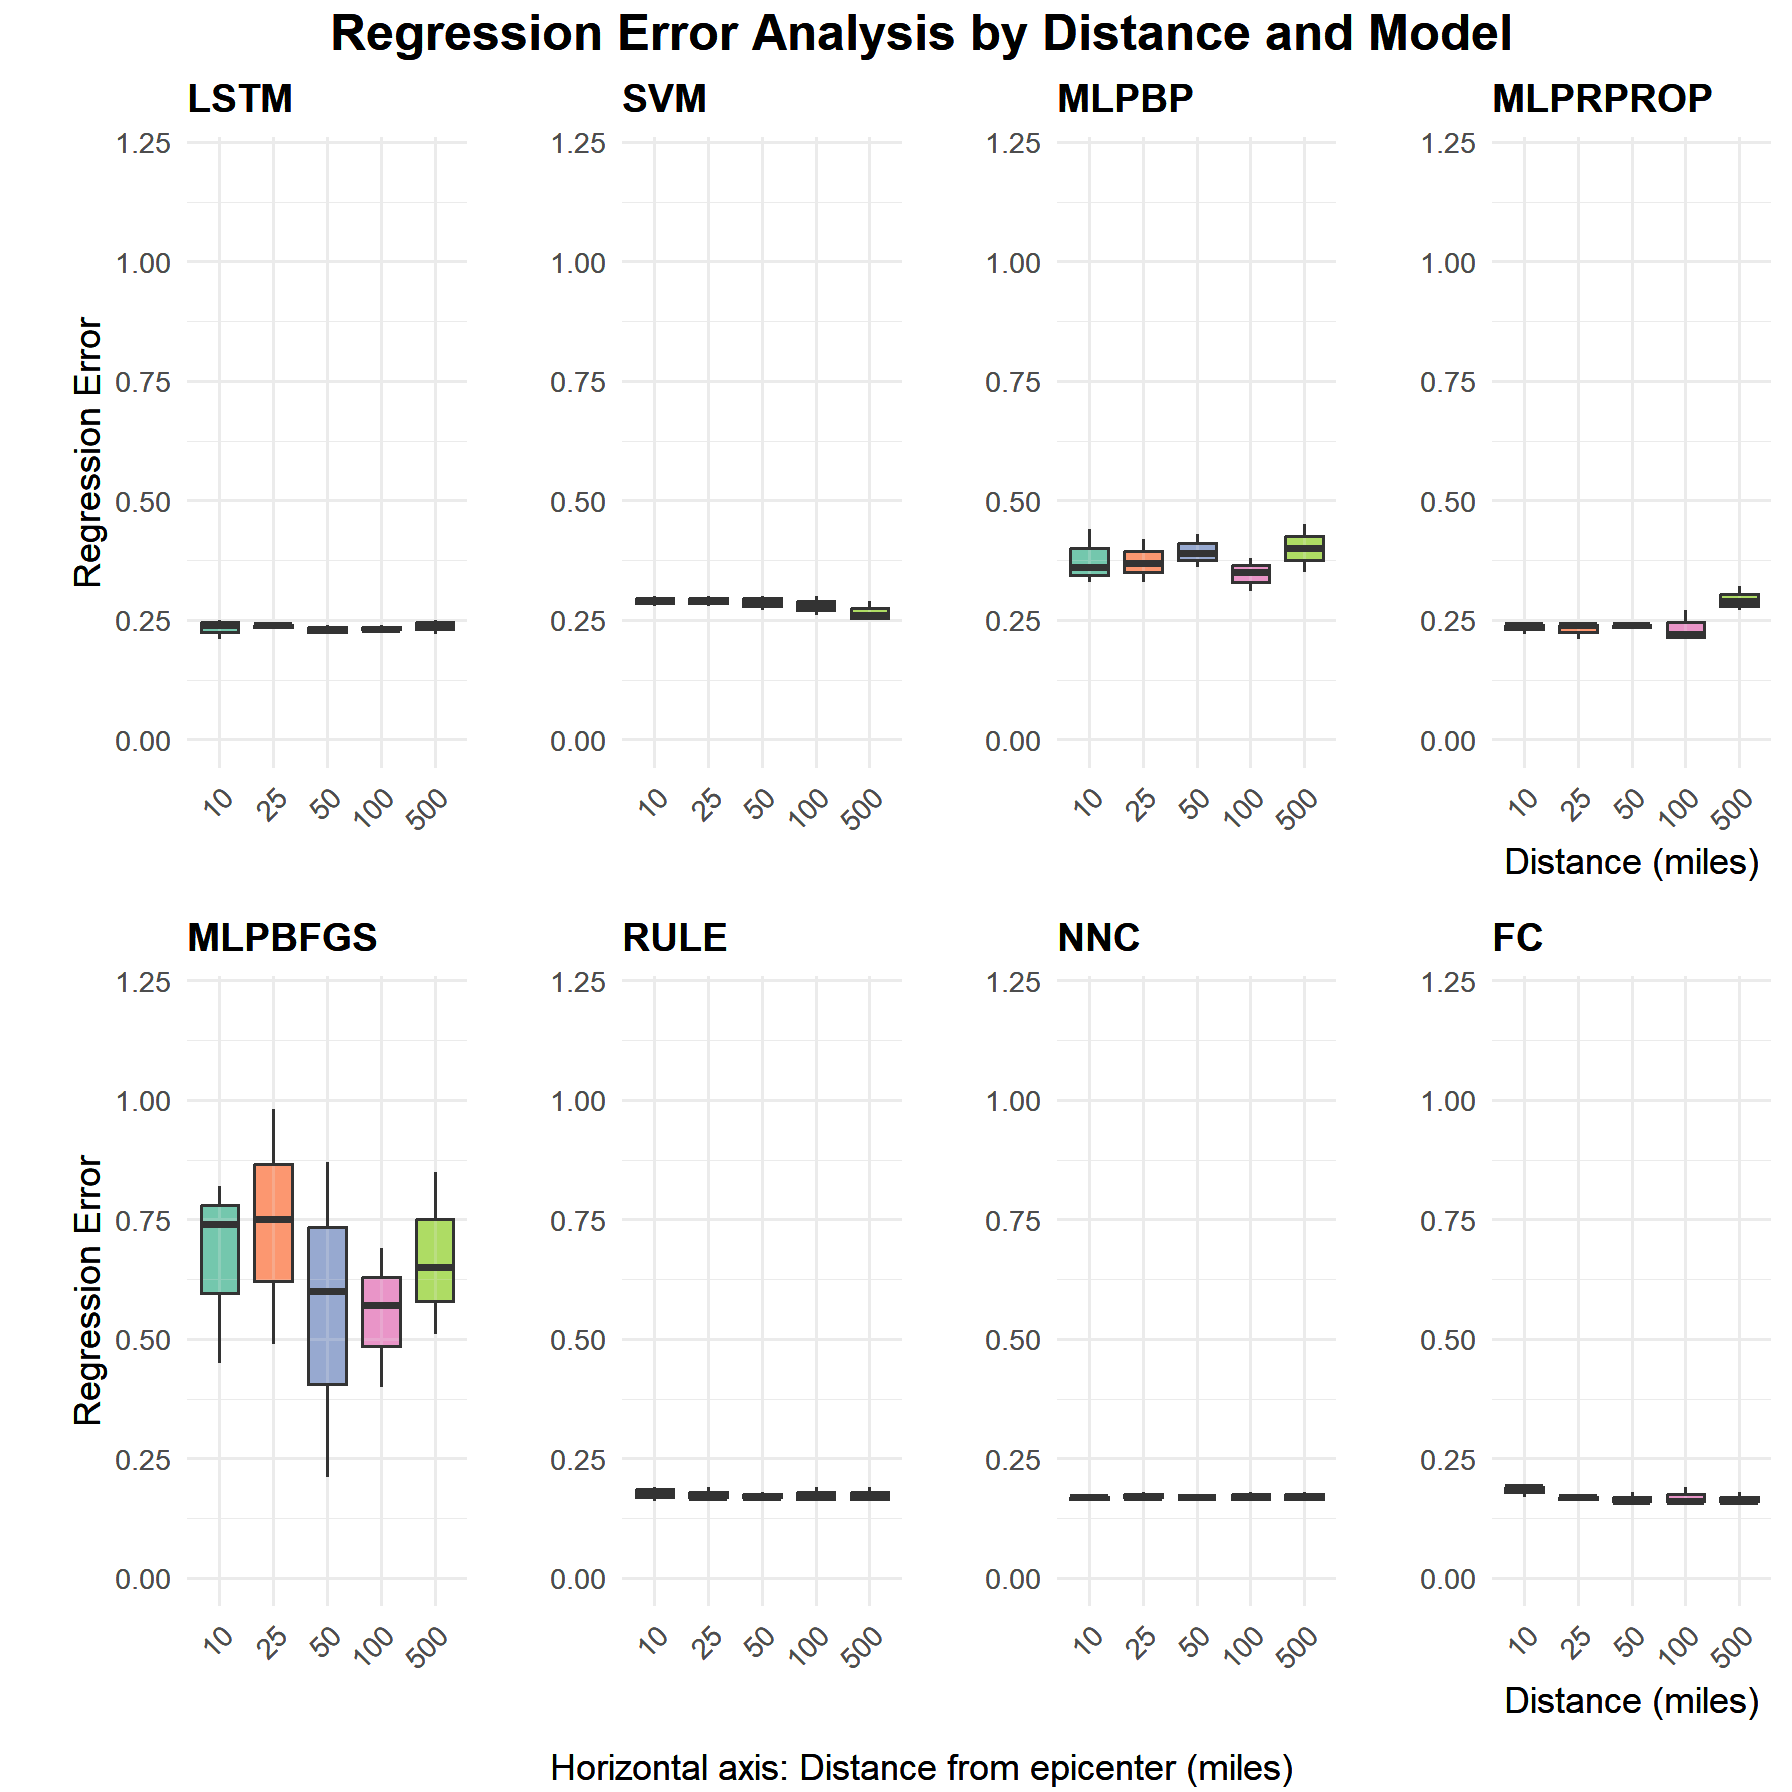
\includegraphics[scale=0.5]{stat2}
\par\end{centering}
\caption{Regression error by distance and model.\label{fig:distanceError}}

\end{figure}

To verify the stability of the application of Grammatical Evolution
to the present seismic data, an additional experiment was performed
where random noise in the range of 0.1\%-5\% was applied to the problem
features one by one. The neural construction method guided by the
Grammatical Evolution was incorporated for the data with the noise
and the average regression error as measured on the test is shown
in Table \ref{tab:noiseResults}. The noise was applied in the results
of the year 2010, where the critical distance $D_{c}$ was set to
10 miles.

\begin{table}[H]

\caption{Experimental results for the year 2010 and $D_{c}=10$ using the Neural
Construction technique. A random noise ranging from 0.001 to 0.05
was applied to the data.\label{tab:noiseResults} The bold notation
is used to indicate the higher test error as measured on the corresponding
test set. }

\centering{}%
\begin{tabular}{|c|c|c|c|c|c|}
\hline 
 & \multicolumn{5}{c|}{NOISE PERCENT}\tabularnewline
\hline 
\hline 
FEATURE & 0.1\% & 0.05\% & 1\% & 2\% & 5\%\tabularnewline
\hline 
1 & 0.176 & \textbf{0.228} & 0.175 & 0.175 & 0.175\tabularnewline
\hline 
2 & \textbf{0.177} & 0.175 & 0.175 & 0.172 & 0.175\tabularnewline
\hline 
3 & 0.175 & \textbf{0.176} & 0.175 & 0.175 & 0.175\tabularnewline
\hline 
4 & \textbf{0.175} & 0.175 & 0.175 & 0.175 & 0.175\tabularnewline
\hline 
5 & \textbf{0.175} & 0.175 & 0.175 & 0.175 & 0.175\tabularnewline
\hline 
6 & 0.175 & \textbf{0.176} & 0.175 & 0.175 & 0.175\tabularnewline
\hline 
7 & 0.175 & 0.175 & 0.175 & \textbf{0.193} & 0.175\tabularnewline
\hline 
8 & \textbf{0.175} & 0.175 & 0.175 & 0.175 & 0.175\tabularnewline
\hline 
9 & \textbf{0.175} & 0.175 & 0.175 & 0.175 & 0.175\tabularnewline
\hline 
10 & \textbf{0.175} & 0.175 & 0.175 & 0.175 & 0.175\tabularnewline
\hline 
11 & 0.175 & 0.175 & 0.175 & 0.175 & \textbf{0.176}\tabularnewline
\hline 
12 & 0.176 & 0.175 & 0.175 & 0.175 & \textbf{0.176}\tabularnewline
\hline 
13 & 0.175 & 0.175 & 0.176 & \textbf{0.176} & 0.175\tabularnewline
\hline 
14 & 0.176 & 0.175 & 0.176 & \textbf{0.176} & 0.175\tabularnewline
\hline 
15 & 0.175 & 0.175 & \textbf{0.176} & 0.175 & 0.175\tabularnewline
\hline 
\end{tabular}
\end{table}
As one can see from the above experimental results, only in a few
cases of noise and only in a limited number of features did a partial
deviation in the error appear compared to the case where there is
no noise in the data.

\section{Conclusions\label{sec:Conclusions}}

The article presents an innovative approach to predicting earthquake
magnitudes using the Grammatical Evolution method, which offers significant
advantages over traditional machine learning techniques. Experimental
results for the years 2004, 2010, and 2012 demonstrate that models
employing grammatical evolution (RULE, NNC, FC) consistently achieve
lower and more stable regression errors compared to models without
grammatical evolution (MLP(BP), MLP(RPROP), MLP(BFGS)). The superiority
of these models is evident both in reducing mean error and in their
resilience to changes in distance, indicating better adaptability
to varying spatial conditions. The study's conclusions emphasize the
capability of grammatical evolution to effectively identify and exploit
structures and relationships in seismic data. Despite the observed
improvement in non-grammatical evolution models over time, their performance
remains inferior to that of models incorporating grammatical evolution.
This demonstrates that using grammatical evolution provides more reliable
predictions, a critical factor for applications such as earthquake
early warning systems.

As future directions, the study suggests exploring the exact mechanisms
through which grammatical evolution enhances performance, focusing
on analyzing the structure of the generated rules. Additionally, the
scalability of the method to larger and more complex datasets could
be investigated, as well as its comparison with other advanced machine
learning techniques. Another avenue could involve optimizing the method's
hyperparameters and incorporating additional geophysical parameters
for even more accurate predictions. Finally, the real-time application
of the model and its integration into early warning frameworks could
be significant steps toward the practical utilization of this research's
findings.

Furthermore, as previously mentioned in the introduction, several
developments of various models have focused on short-term early warning
systems, typically offering a lead time of approximately one minute,
based on real-time detection of tectonic or lithospheric plate movement
as it occurs. In contrast, our study not only targets seismic events
of magnitude 5.0 and above, but also takes a step further by demonstrating
the potential to predict such events before any plate movement is
detected. Consequently, our model can potentially be integrated into
a broader early warning framework capable of delivering mid to long-term
predictions of earthquake occurrences, ranging from hours or days
to even months in advance, thereby offering a significantly enhanced
preparedness window, and risk mitigation efforts.

\authorcontributions{C.K., V.C. and I.G.T. conceived of the idea and the methodology,
and C.K. and V.C. implemented the corresponding software. C.K. conducted
the experiments, employing objective functions as test cases, and
provided the comparative experiments. V.C. performed the necessary
statistical tests. All authors have read and agreed to the published
version of the manuscript.}

\funding{This research has been financed by the European Union : Next Generation
EU through the Program Greece 2.0 National Recovery and Resilience
Plan , under the call RESEARCH -- CREATE -- INNOVATE, project name
“iCREW: Intelligent small craft simulator for advanced crew training
using Virtual Reality techniques\textquotedbl{} (project code:TAEDK-06195).
\quad{}}

\institutionalreview{Not applicable.}

\informedconsent{Not applicable.}

\dataavailability{Data are contained within the article.}

\conflictsofinterest{The authors declare no conflicts of interest.}

\begin{adjustwidth}{-\extralength}{0cm}{}


\reftitle{References}
\begin{thebibliography}{999}
\bibitem[Author1(1989)]{britanica} Seismograph. Britannica, Earth
Sciences. Available from: \url{https://www.britannica.com/science/seismograph }(accessed
on 20 May 2025).

\bibitem[(1989)]{britanica2}Robert Mallet. Britannica, Civil Engineering.
Available from: \url{https://www.britannica.com/biography/Robert-Mallet}
(accessed on 20 May 2025).

\bibitem[(1989)]{geological}Can you predict earthquakes? United States
Geological Survey. Available from: \url{https://www.usgs.gov/faqs/can-you-predict-earthquakes}
(accessed on 20 May 2025).

\bibitem[(1989)]{Bergen}Bergen, K. J., Chen, T., \& Li, Z. (2019).
Preface to the focus section on machine learning in seismology. Seismological
Research Letters, 90(2A), 477-480.

\bibitem[(1989)]{Hutchison}How machine learning might unlock earthquake
prediction. MIT Technology Review, article by: Allie Hutchison. Published
on: December 29, 2023. Available from: \url{https://www.technologyreview.com/2023/12/29/1084699/machine-learning-earthquake-prediction-ai-artificial-intelligence/}
(accessed on 20 May 2025).

\bibitem[(1989)]{Hincks}Hincks, T., Aspinall, W., Cooke, R., \& Gernon,
T. (2018). Oklahoma's induced seismicity strongly linked to wastewater
injection depth. Science, 359(6381), 1251-1255.

\bibitem[(1989)]{obara2022}Obara, K. (2002). Nonvolcanic deep tremor
associated with subduction in southwest Japan. Science, 296(5573),
1679-1681.

\bibitem[(1989)]{obara2016}Obara, K., \& Kato, A. (2016). Connecting
slow earthquakes to huge earthquakes. Science, 353(6296), 253-257.

\bibitem[(1989)]{bletery}Bletery, Q., \& Nocquet, J. M. (2023). The
precursory phase of large earthquakes. Science, 381(6655), 297-301.

\bibitem[(1989)]{planc}The secret knowledge of animals. Max Planck
Institute of Animal Behavior. Published on: April 12 2024. Available
from: \url{https://www.ab.mpg.de/578863/news_publication_21821500_transferred?c=413930}
(accessed on 20 May 2025).

\bibitem[(1989)]{mousavi}Mousavi, S. M., \& Beroza, G. C. (2020).
A machine‐learning approach for earthquake magnitude estimation. Geophysical
Research Letters, 47(1), e2019GL085976.

\bibitem[(1989)]{devries}DeVries, P. M., Viégas, F., Wattenberg,
M., \& Meade, B. J. (2018). Deep learning of aftershock patterns following
large earthquakes. Nature, 560(7720), 632-634.

\bibitem[(1989)]{ross}Ross, Z. E., Meier, M. A., \& Hauksson, E.
(2018). P wave arrival picking and first‐motion polarity determination
with deep learning. Journal of Geophysical Research: Solid Earth,
123(6), 5120-5129.

\bibitem[(1989)]{rouet}Rouet‐Leduc, B., Hulbert, C., Lubbers, N.,
Barros, K., Humphreys, C. J., \& Johnson, P. A. (2017). Machine learning
predicts laboratory earthquakes. Geophysical Research Letters, 44(18),
9276-9282.

\bibitem[(1989)]{rouet2019}Rouet-Leduc, B., Hulbert, C., \& Johnson,
P. A. (2019). Continuous chatter of the Cascadia subduction zone revealed
by machine learning. Nature Geoscience, 12(1), 75-79.

\bibitem[(1989)]{tan}Tan, Y. J., Waldhauser, F., Ellsworth, W. L.,
Zhang, M., Zhu, W., Michele, M., ... \& Segou, M. (2021). Machine‐learning‐based
high‐resolution earthquake catalog reveals how complex fault structures
were activated during the 2016--2017 central Italy sequence. The
Seismic Record, 1(1), 11-19.

\bibitem[(1989)]{mousavi2020}Mousavi, S. M., Ellsworth, W. L., Zhu,
W., Chuang, L. Y., \& Beroza, G. C. (2020). Earthquake transformer---an
attentive deep-learning model for simultaneous earthquake detection
and phase picking. Nature communications, 11(1), 3952.

\bibitem[(1989)]{hsu}Hsu, Y. F., Zaliapin, I., \& Ben‐Zion, Y. (2024).
Informative modes of seismicity in nearest‐neighbor earthquake proximities.
Journal of Geophysical Research: Solid Earth, 129(3), e2023JB027826.

\bibitem[(1989)]{bayliss}Bayliss, K., Naylor, M., \& Main, I. G.
(2019). Probabilistic identification of earthquake clusters using
rescaled nearest neighbour distance networks. Geophysical Journal
International, 217(1), 487-503.

\bibitem[(1989)]{saad}Saad, O. M., Chen, Y., Savvaidis, A., Fomel,
S., Jiang, X., Huang, D., ... \& Chen, Y. (2023). Earthquake forecasting
using big data and artificial intelligence: A 30‐week real‐time case
study in China. Bulletin of the Seismological Society of America,
113(6), 2461-2478.

\bibitem[(1989)]{asim}Asim, K. M., Martínez-Álvarez, F., Basit, A.,
\& Iqbal, T. (2017). Earthquake magnitude prediction in Hindukush
region using machine learning techniques. Natural Hazards, 85, 471-486.

\bibitem[(1989)]{corbi}Corbi, F., Sandri, L., Bedford, J., Funiciello,
F., Brizzi, S., Rosenau, M., \& Lallemand, S. (2019). Machine learning
can predict the timing and size of analog earthquakes. Geophysical
Research Letters, 46(3), 1303-1311.

\bibitem[(1989)]{hoque}Hoque, A., Raj, J., Saha, A., \& Bhattacharya,
P. (2020). Earthquake magnitude prediction using machine learning
technique. In Trends in Computational Intelligence, Security and Internet
of Things: Third International Conference, ICCISIoT 2020, Tripura,
India, December 29-30, 2020, Proceedings 3 (pp. 37-53). Springer International
Publishing.

\bibitem[(1989)]{zhu}Zhu, C., Cotton, F., Kawase, H., \& Nakano,
K. (2023). How well can we predict earthquake site response so far?
Machine learning vs physics-based modeling. Earthquake Spectra, 39(1),
478-504.

\bibitem[(1989)]{xiong}Xiong, P., Tong, L., Zhang, K., Shen, X.,
Battiston, R., Ouzounov, D., ... \& Zhou, H. (2021). Towards advancing
the earthquake forecasting by machine learning of satellite data.
Science of the Total Environment, 771, 145256.

\bibitem[(2023)]{bhatia}Bhatia, M., Ahanger, T. A., \& Manocha, A.
(2023). Artificial intelligence based real-time earthquake prediction.
Engineering Applications of Artificial Intelligence, 120, 105856.

\bibitem[(2023)]{japan}Earthquake Early Warning System. Japan Meteorological
Agency. Available from:\url{ https://www.jma.go.jp/jma/en/Activities/eew.html}
(accessed on 20 May 2025).

\bibitem[(2023)]{wikipedia}Earthquake Early Warning System (Japan).
Wikipedia. Available from: \url{https://en.wikipedia.org/wiki/Earthquake_Early_Warning_(Japan)}
(accessed on 20 May 2025).

\bibitem[(2023)]{us_survey}ShakeAlert. US Geological Survey, Earthquake
Hazards Program. Available from: \url{https://earthquake.usgs.gov/data/shakealert/}
(accessed on 20 May 2025).

\bibitem[(2023)]{shakealert}ShakeAlert. Earthquake Early Warning
(EEW) System. Available from:\url{ https://www.shakealert.org/} (accessed
on 20 May 2025).

\bibitem[(2023)]{beroza}Beroza, G. C., Segou, M., \& Mostafa Mousavi,
S. (2021). Machine learning and earthquake forecasting---next steps.
Nature communications, 12(1), 4761.

\bibitem[(2023)]{mousavi_review}Mousavi, S. M., \& Beroza, G. C.
(2023). Machine learning in earthquake seismology. Annual Review of
Earth and Planetary Sciences, 51(1), 105-129.

\bibitem{ge1}M. O’Neill, C. Ryan, Grammatical evolution, IEEE Trans.
Evol. Comput. \textbf{5,}pp. 349--358, 2001.

\bibitem[(year)]{bnf1}J. W. Backus. The Syntax and Semantics of the
Proposed International Algebraic Language of the Zurich ACM-GAMM Conference.
Proceedings of the International Conference on Information Processing,
UNESCO, 1959, pp.125-132.

\bibitem{ge_program1}C. Ryan, J. Collins, M. O’Neill, Grammatical
evolution: Evolving programs for an arbitrary language. In: Banzhaf,
W., Poli, R., Schoenauer, M., Fogarty, T.C. (eds) Genetic Programming.
EuroGP 1998. Lecture Notes in Computer Science, vol 1391. Springer,
Berlin, Heidelberg, 1998.

\bibitem{ge_program2}M. O’Neill, M., C. Ryan, Evolving Multi-line
Compilable C Programs. In: Poli, R., Nordin, P., Langdon, W.B., Fogarty,
T.C. (eds) Genetic Programming. EuroGP 1999. Lecture Notes in Computer
Science, vol 1598. Springer, Berlin, Heidelberg, 1999.

\bibitem{ge_music}A.O. Puente, R. S. Alfonso, M. A. Moreno, Automatic
composition of music by means of grammatical evolution, In: APL '02:
Proceedings of the 2002 conference on APL: array processing languages:
lore, problems, and applications July 2002 Pages 148--155. 

\bibitem{ge_pacman}E. Galván-López, J.M. Swafford, M. O’Neill, A.
Brabazon, Evolving a Ms. PacMan Controller Using Grammatical Evolution.
In: , et al. Applications of Evolutionary Computation. EvoApplications
2010. Lecture Notes in Computer Science, vol 6024. Springer, Berlin,
Heidelberg, 2010.

\bibitem{ge_supermario}N. Shaker, M. Nicolau, G. N. Yannakakis, J.
Togelius, M. O'Neill, Evolving levels for Super Mario Bros using grammatical
evolution, 2012 IEEE Conference on Computational Intelligence and
Games (CIG), 2012, pp. 304-31.

\bibitem{ge_energy}D. Martínez-Rodríguez, J. M. Colmenar, J. I. Hidalgo,
R.J. Villanueva Micó, S. Salcedo-Sanz, Particle swarm grammatical
evolution for energy demand estimation, Energy Science and Engineering
\textbf{8}, pp. 1068-1079, 2020.

\bibitem{ge_crypt}C. Ryan, M. Kshirsagar, G. Vaidya, G. et al. Design
of a cryptographically secure pseudo random number generator with
grammatical evolution. Sci Rep \textbf{12}, 8602, 2022.

\bibitem{ge_trading}C. Martín, D. Quintana, P. Isasi, Grammatical
Evolution-based ensembles for algorithmic trading, Applied Soft Computing
\textbf{84}, 105713, 2019.

\bibitem[(2020)]{nn1}C. Bishop, Neural Networks for Pattern Recognition,
Oxford University Press, 1995.

\bibitem{nn2}G. Cybenko, Approximation by superpositions of a sigmoidal
function, Mathematics of Control Signals and Systems \textbf{2}, pp.
303-314, 1989.

\bibitem[(1994)]{neural_quake}Lakkos S, Hadjiprocopis A, Compley
R, Smith P (1994) A neural network scheme for earthquake prediction
based on the Seismic Electric Signals. In: Proceedings of the IEEE
conference on neural networks and signal processing, Ermioni, 681-689. 

\bibitem[(1994)]{layered_quake}Negarestani A, Setayeshi S, Ghannadi-Maragheh
M, Akashe B (2002) Layered neural networks based analysis of radon
concentration and environmental parameters in earthquake prediction.
J. Environmental Radioactivity 62:225-233.

\bibitem[(1994)]{neural_magnitude}Panakkat A, Adeli H (2007) Neural
network models for earthquake magnitude prediction using multiple
seismicity indicators. Int. J. Neural Systems 17:13-33

\bibitem[(1994)]{gen1}Holland, J. H. (1992). Genetic algorithms.
Scientific american, 267(1), 66-73.

\bibitem[(1994)]{gen2}Sastry, K., Goldberg, D., \& Kendall, G. (2005).
Genetic algorithms. Search methodologies: Introductory tutorials in
optimization and decision support techniques, 97-125.

\bibitem{rule_tsoulos}I.G. Tsoulos, Learning Functions and Classes
Using Rules, AI. \textbf{3}, pp.751-763, 2022. 

\bibitem[(2008)]{nnc}I.G. Tsoulos, D. Gavrilis, E. Glavas, Neural
network construction and training using grammatical evolution, Neurocomputing
\textbf{72}, pp. 269-277, 2008.

\bibitem{nnc_amide1}G.V. Papamokos, I.G. Tsoulos, I.N. Demetropoulos,
E. Glavas, Location of amide I mode of vibration in computed data
utilizing constructed neural networks, Expert Systems with Applications
\textbf{36}, pp. 12210-12213, 2009.

\bibitem{nnc_student}V. Christou, I.G. Tsoulos, V. Loupas, A.T. Tzallas,
C. Gogos, P.S. Karvelis, N. Antoniadis, E. Glavas, N. Giannakeas,
Performance and early drop prediction for higher education students
using machine learning, Expert Systems with Applications \textbf{225},
120079, 2023.

\bibitem{nnc_autism}E.I. Toki, J. Pange, G. Tatsis, K. Plachouras,
I.G. Tsoulos, Utilizing Constructed Neural Networks for Autism Screening,
Applied Sciences \textbf{14}, 3053, 2024.

\bibitem[(2008)]{fc1}Dimitris Gavrilis, Ioannis G. Tsoulos, Evangelos
Dermatas, Selecting and constructing features using grammatical evolution,
Pattern Recognition Letters \textbf{29},pp. 1358-1365, 2008. 

\bibitem[(2008)]{rbf1}J. Park and I. W. Sandberg, Universal Approximation
Using Radial-Basis-Function Networks, Neural Computation 3, pp. 246-257,
1991.

\bibitem{rbf2}H. Yu, T. Xie, S. Paszczynski, B. M. Wilamowski, Advantages
of Radial Basis Function Networks for Dynamic System Design, in IEEE
Transactions on Industrial Electronics \textbf{58}, pp. 5438-5450,
2011.

\bibitem[(2009)]{weka_main}M. Hall, F. Frank, G. Holmes, B. Pfahringer,
P. Reutemann, I.H. Witten, The WEKA data mining software: an update.
ACM SIGKDD explorations newsletter \textbf{11}, pp. 10-18, 2009.

\bibitem[(2022)]{nnc_softx}Tsoulos, I. G., Tzallas, A., \& Tsalikakis,
D. (2019). NNC: A tool based on Grammatical Evolution for data classification
and differential equation solving. SoftwareX, 10, 100297.

\bibitem[(2022)]{qfc}I.G. Tsoulos, QFC: A Parallel Software Tool
for Feature Construction, Based on Grammatical Evolution, Algorithms
\textbf{15}, 295, 2022.

\bibitem[(2019)]{lstm}Yu, Y., Si, X., Hu, C., \& Zhang, J. (2019).
A review of recurrent neural networks: LSTM cells and network architectures.
Neural computation, 31(7), 1235-1270.

\bibitem[(2021)]{pytorch}Ketkar, N., Moolayil, J., Ketkar, N., \&
Moolayil, J. (2021). Introduction to pytorch. Deep learning with python:
learn best practices of deep learning models with PyTorch, 27-91.

\bibitem[(2009)]{svm}Xue, H., Yang, Q., \& Chen, S. (2009). SVM:
Support vector machines. In The top ten algorithms in data mining
(pp. 51-74). Chapman and Hall/CRC.

\bibitem[(2009)]{libsvm}Chang, C. C., \& Lin, C. J. (2011). LIBSVM:
a library for support vector machines. ACM transactions on intelligent
systems and technology (TIST), 2(3), 1-27.

\bibitem{bpnn1}Vora, K., \& Yagnik, S. (2014). A survey on backpropagation
algorithms for feedforward neural networks. International Journal
of Engineering Development and Research, 1(3), 193-197.

\bibitem{bpnn2}K. Vora, S. Yagnik, A survey on backpropagation algorithms
for feedforward neural networks, International Journal of Engineering
Development and Research \textbf{1}, pp. 193-197, 2014.

\bibitem{rpropnn-1}Pajchrowski, T., Zawirski, K., \& Nowopolski,
K. (2014). Neural speed controller trained online by means of modified
RPROP algorithm. IEEE transactions on industrial informatics, 11(2),
560-568.

\bibitem{rpropnn-2}Hermanto, R. P. S., \& Nugroho, A. (2018). Waiting-time
estimation in bank customer queues using RPROP neural networks. Procedia
Computer Science, 135, 35-42.

\bibitem{powell}M.J.D Powell, A Tolerant Algorithm for Linearly Constrained
Optimization Calculations, Mathematical Programming \textbf{45}, pp.
547-566, 1989. 

\end{thebibliography}
%%%%%%%%%%%%%%%%%%%%%%%%%%%%%%%%%%%%%%%%%%
%% for journal Sci
%\reviewreports{\\
%Reviewer 1 comments and authors' response\\
%Reviewer 2 comments and authors' response\\
%Reviewer 3 comments and authors' response
%}
%%%%%%%%%%%%%%%%%%%%%%%%%%%%%%%%%%%%%%%%%%

\PublishersNote{}

\end{adjustwidth}{}
\end{document}
